\documentclass[
    xcolor={svgnames,dvipsnames},
    hyperref={colorlinks, citecolor=DeepPink4, linkcolor=DarkRed, urlcolor=DarkBlue}
    ]{beamer}  % for hardcopy add 'trans'

\mode<presentation>
{
  \usetheme{Singapore}
  % or ...
  \setbeamercovered{transparent}
  % or whatever (possibly just delete it)
}



\addtobeamertemplate{navigation symbols}{}{%
    \usebeamerfont{footline}%
    \usebeamercolor[fg]{footline}%
    \hspace{1em}%
    \insertframenumber/\inserttotalframenumber
}



\usepackage{fontspec} 
%\usepackage[xcharter]{newtxmath}
%\setmainfont{XCharter}
\usepackage{unicode-math}
%\setmathfont{XCharter-Math.otf}
\setmonofont{DejaVu Sans Mono}[Scale=MatchLowercase] % provides unicode characters 

\usepackage{tikz}
\usetikzlibrary{shadows, trees, shapes.geometric, matrix, shapes, arrows.meta, positioning, fit, backgrounds, calc}

% \usetikzlibrary{matrix, arrows.meta, positioning, calc, backgrounds}

% for tikz
\usepackage{pgfplots}
\usepgfplotslibrary{fillbetween}
\pgfplotsset{compat=1.16}

\usepackage{varwidth}
\usepackage{minted}
\usemintedstyle{friendly}
\setminted[python]{
  fontsize=\small,
  baselinestretch=1.2,
  bgcolor=codebg,
  linenos=false,
  breaklines=true,
  frame=none
}
\setminted[matlab]{
  fontsize=\small,
  baselinestretch=1.2,
  bgcolor=codebg,
  linenos=false,
  breaklines=true,
  frame=none
}
\setminted[julia]{
  fontsize=\small,
  baselinestretch=1.2,
  bgcolor=codebg,
  linenos=false,
  breaklines=true,
  frame=none
}
%\setminted{mathescape, frame=lines, framesep=3mm}
%\newminted{python}{}
%\newminted{c}{mathescape,frame=lines,framesep=4mm,bgcolor=bg}
%\newminted{java}{mathescape,frame=lines,framesep=4mm,bgcolor=bg}
%\newminted{julia}{mathescape,frame=lines,framesep=4mm,bgcolor=bg}
%\newminted{ipython}{mathescape,frame=lines,framesep=4mm,bgcolor=bg}

\usepackage{graphicx}
\usepackage{amsmath, amssymb, amsthm}
\usepackage{bbm}
\usepackage{mathrsfs}
\usepackage{xcolor}
\usepackage{fancyvrb}


% Quotes at start of chapters / sections
\usepackage{epigraph}  
\renewcommand{\epigraphwidth}{6in}

%% Fonts

%\usepackage[T1]{fontenc}
\usepackage{mathpazo}
%\usepackage{fontspec}
%\defaultfontfeatures{Ligatures=TeX}
%\setsansfont[Scale=MatchLowercase]{DejaVu Sans}
%\setmonofont[Scale=MatchLowercase]{DejaVu Sans Mono}
%\setmathfont{Asana Math}
%\setmainfont{Optima}
%\setmathrm{Optima}
%\setboldmathrm[BoldFont={Optima ExtraBlack}]{Optima Bold}

% Some colors

\definecolor{containerblue}{RGB}{66, 133, 244}
\definecolor{leafgreen}{RGB}{52, 168, 83}
\definecolor{textgray}{RGB}{51, 51, 51}
\definecolor{backgroundgray}{RGB}{248, 249, 250}
\definecolor{codebg}{RGB}{241, 241, 241}
\definecolor{aquamarine}{RGB}{69,139,116}
\definecolor{midnightblue}{RGB}{25,25,112}
\definecolor{darkslategrey}{RGB}{47,79,79}
\definecolor{darkorange4}{RGB}{139,90,0}
\definecolor{dogerblue}{RGB}{24,116,205}
\definecolor{blue2}{RGB}{0,0,238}
\definecolor{bg}{rgb}{0.95,0.95,0.95}
\definecolor{DarkOrange1}{RGB}{255,127,0}
\definecolor{ForestGreen}{RGB}{34,139,34}
\definecolor{DarkRed}{RGB}{139, 0, 0}
\definecolor{DarkBlue}{RGB}{0, 0, 139}
\definecolor{Blue}{RGB}{0, 0, 255}
\definecolor{Brown}{RGB}{165,42,42}


\setlength{\parskip}{1.5ex plus0.5ex minus0.5ex}

%\renewcommand{\baselinestretch}{1.05}
%\setlength{\parskip}{1.5ex plus0.5ex minus0.5ex}
%\setlength{\parindent}{0pt}

% Typesetting code
\definecolor{bg}{rgb}{0.95,0.95,0.95}
\newcommand{\Fact}{\textcolor{Brown}{\bf Fact. }}
\newcommand{\Facts}{\textcolor{Brown}{\bf Facts }}
\newcommand{\keya}{\textcolor{turquois4}{\bf Key Idea. }}
\newcommand{\Factnodot}{\textcolor{Brown}{\bf Fact }}
\newcommand{\Eg}{\textcolor{ForestGreen}{Example. }}
\newcommand{\Egs}{\textcolor{ForestGreen}{Examples. }}
\newcommand{\Ex}{{\bf Ex. }}



\renewcommand{\theFancyVerbLine}{\sffamily
    \textcolor[rgb]{0.5,0.5,1.0}{\scriptsize {\arabic{FancyVerbLine}}}}

\newcommand{\navy}[1]{\textcolor{DarkBlue}{\bf #1}}
\newcommand{\brown}[1]{\textcolor{Brown}{\sf #1}}
\newcommand{\green}[1]{\textcolor{ForestGreen}{\sf #1}}
\newcommand{\blue}[1]{\textcolor{Blue}{\sf #1}}
\newcommand{\emp}[1]{\textcolor{Maroon}{\bf #1}}
\newcommand{\red}[1]{\textcolor{Red}{\bf #1}}

% Symbols, redefines, etc.

\newcommand{\code}[1]{\texttt{#1}}

\newcommand{\argmax}{\operatornamewithlimits{argmax}}
\newcommand{\argmin}{\operatornamewithlimits{argmin}}

\DeclareMathOperator{\cl}{cl}
\DeclareMathOperator{\interior}{int}
\DeclareMathOperator{\Prob}{Prob}
\DeclareMathOperator{\determinant}{det}
\DeclareMathOperator{\trace}{trace}
\DeclareMathOperator{\Span}{span}
\DeclareMathOperator{\rank}{rank}
\DeclareMathOperator{\cov}{cov}
\DeclareMathOperator{\corr}{corr}
\DeclareMathOperator{\var}{var}
\DeclareMathOperator{\mse}{mse}
\DeclareMathOperator{\se}{se}
\DeclareMathOperator{\row}{row}
\DeclareMathOperator{\col}{col}
\DeclareMathOperator{\range}{rng}
\DeclareMathOperator{\dimension}{dim}
\DeclareMathOperator{\bias}{bias}


% mics short cuts and symbols
\newcommand{\st}{\ensuremath{\ \mathrm{s.t.}\ }}
\newcommand{\setntn}[2]{ \{ #1 : #2 \} }
\newcommand{\cf}[1]{ \lstinline|#1| }
\newcommand{\fore}{\therefore \quad}
\newcommand{\tod}{\stackrel { d } {\to} }
\newcommand{\toprob}{\stackrel { p } {\to} }
\newcommand{\toms}{\stackrel { ms } {\to} }
\newcommand{\eqdist}{\stackrel {\textrm{ \scriptsize{d} }} {=} }
\newcommand{\iidsim}{\stackrel {\textrm{ {\sc iid }}} {\sim} }
\newcommand{\1}{\mathbbm 1}
\newcommand{\dee}{\,{\rm d}}
\newcommand{\given}{\, | \,}
\newcommand{\la}{\langle}
\newcommand{\ra}{\rangle}

\newcommand{\boldA}{\mathbf A}
\newcommand{\boldB}{\mathbf B}
\newcommand{\boldC}{\mathbf C}
\newcommand{\boldD}{\mathbf D}
\newcommand{\boldM}{\mathbf M}
\newcommand{\boldP}{\mathbf P}
\newcommand{\boldQ}{\mathbf Q}
\newcommand{\boldI}{\mathbf I}
\newcommand{\boldX}{\mathbf X}
\newcommand{\boldY}{\mathbf Y}
\newcommand{\boldZ}{\mathbf Z}

\newcommand{\bSigmaX}{ {\boldsymbol \Sigma_{\hboldbeta}} }
\newcommand{\hbSigmaX}{ \mathbf{\hat \Sigma_{\hboldbeta}} }

\newcommand{\RR}{\mathbbm R}
\newcommand{\NN}{\mathbbm N}
\newcommand{\PP}{\mathbbm P}
\newcommand{\EE}{\mathbbm E \,}
\newcommand{\XX}{\mathbbm X}
\newcommand{\ZZ}{\mathbbm Z}
\newcommand{\QQ}{\mathbbm Q}

\newcommand{\fF}{\mathcal F}
\newcommand{\dD}{\mathcal D}
\newcommand{\lL}{\mathcal L}
\newcommand{\gG}{\mathcal G}
\newcommand{\hH}{\mathcal H}
\newcommand{\nN}{\mathcal N}
\newcommand{\pP}{\mathcal P}

\definecolor{jaxblue}{HTML}{4285F4}
\definecolor{xlagreen}{HTML}{34A853}
\definecolor{pythonorange}{HTML}{FF6F00}
\definecolor{devicegray}{HTML}{607D8B}
\definecolor{compilerpurple}{HTML}{8E24AA}
\definecolor{tracingyellow}{HTML}{FBBC04}



\title{Computational Economics and the AI Revolution}



\author{John Stachurski}


\date{2025}


\begin{document}

\begin{frame}
  \titlepage
\end{frame}



\begin{frame}{Topics}

    \begin{enumerate}
        \item The AI revolution
        \vspace{0.5em}
        \item ANNs and deep learning
        \vspace{0.5em}
        \item AI software and hardware
        \vspace{0.5em}
        \item Can we use this for econ?
        \vspace{0.5em}
        \item Applications
    \end{enumerate}

\end{frame}

\begin{frame}
    
    The aim of this lecture is \brown{limited}
    \medskip


    \begin{itemize}
        \item Better understanding of core AI methods / tools
        \medskip
        \item How can this knowledge be applied to economic modeling today?
    \end{itemize}

    \medskip
    \medskip
    Focus is \brown{technical}
    \medskip


    \begin{itemize}
        \item Build understanding of maths / stats / code
    \end{itemize}

\end{frame}




\begin{frame}{The AI revolution}


    \begin{itemize}
        \item generative AI 
        \vspace{0.5em}
        \item image processing / computer vision
        \vspace{0.5em}
        \item speech recognition
        \vspace{0.5em}
        \item translation
        \vspace{0.5em}
        \item scientific knowledge discovery
        \vspace{0.5em}
        \item forecasting and prediction 
        \vspace{0.5em}
        \item etc.
    \end{itemize}

    
\end{frame}

\begin{frame}{Example: AlphaEvolve} 

    A coding agent for scientific and algorithmic knowledge discovery

    \medskip

    \begin{figure}
       \centering
       \scalebox{0.24}{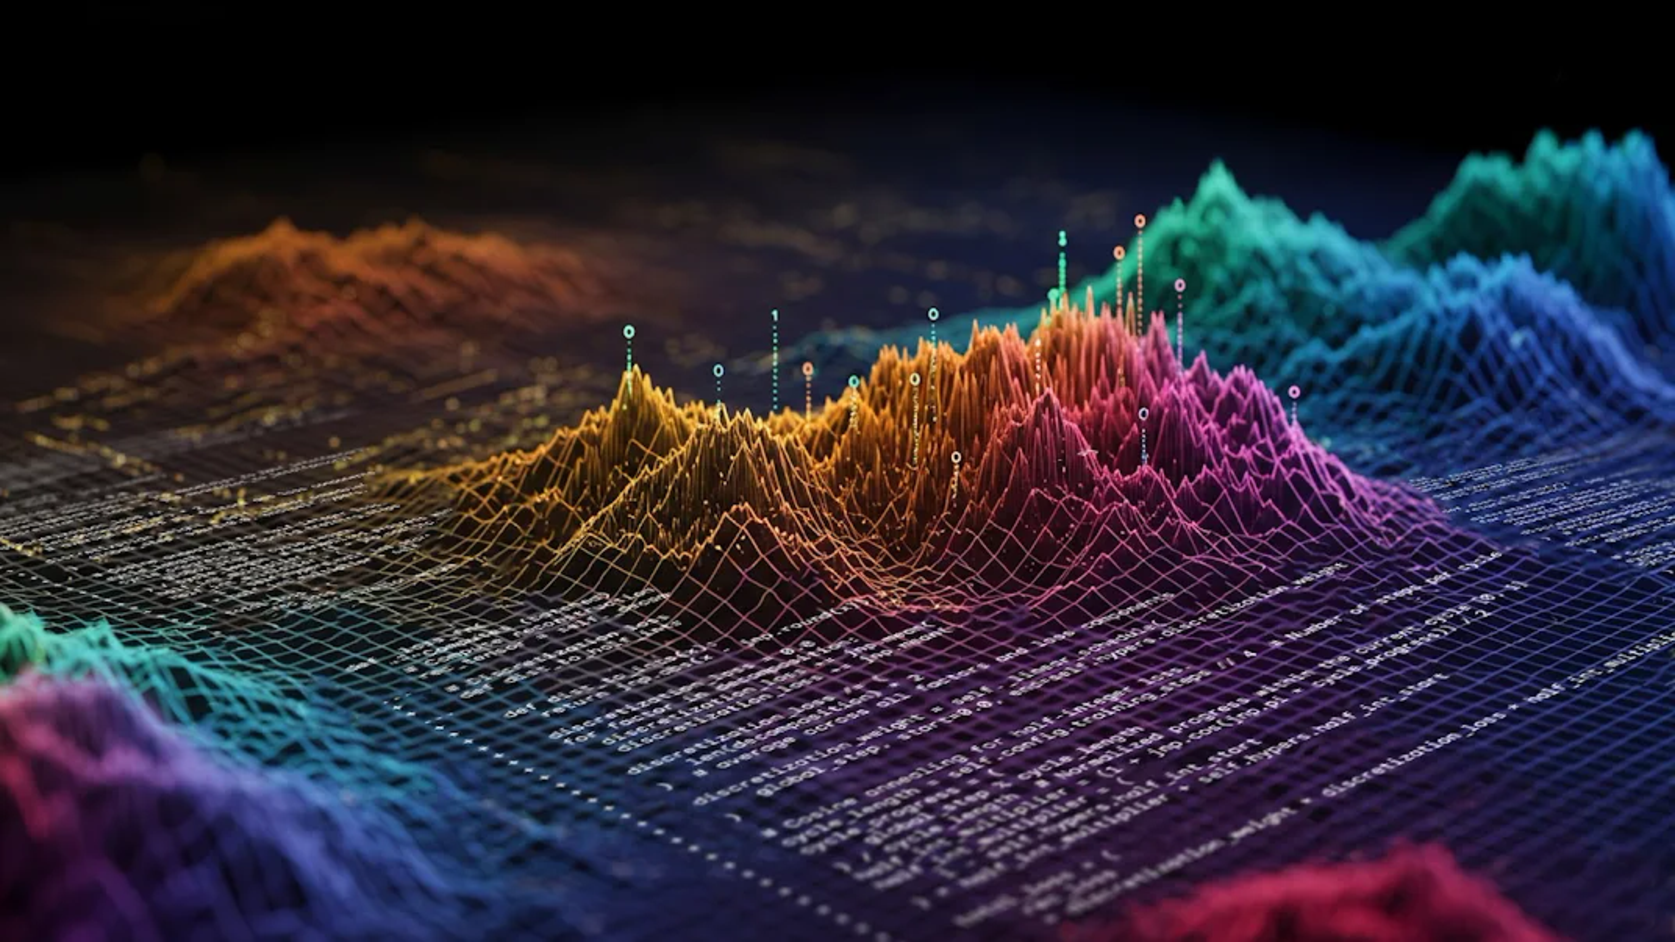
\includegraphics[trim={0cm 0cm 0cm 0cm},clip]{evolve.pdf}}
    \end{figure}

    \begin{center}
        Google Deepmind (May 2025)
    \end{center}

\end{frame}

\begin{frame}
    
    Develops algorithms and code using an ensemble of LLMs

    \vspace{0.5em}
    \begin{itemize}
        \item Test, iterate, refine
    \end{itemize}

    \vspace{0.5em}
    \vspace{0.5em}
    \vspace{0.5em}
    Employs an \brown{evolutionary algorithm}

    \vspace{0.5em}
    \begin{itemize}
        \item Promising solutions are selected and mutated by LLMs 
        \vspace{0.5em}
        \item ``Survival of the fittest" progressively improves performance
    \end{itemize}

        \vspace{0.5em}
        \vspace{0.5em}
    Discovered a new matrix multiplication algorithm

    \begin{itemize}
        \item Surpasses Strassen's algorithm for 4x4 matrices
        \vspace{0.5em}
        \item Breaks a 56 year old record
    \end{itemize}

\end{frame}


\begin{frame}\frametitle{Example: AlphaFold}
    
    \begin{figure}
       \centering
       \scalebox{0.2}{
\includegraphics[trim={0cm 0cm 0cm 0cm},clip]{alpha_fold.pdf}}
    \end{figure}

\end{frame}

\begin{frame}

    \begin{itemize}
        \item Developed by Google DeepMind 
            \vspace{0.5em}
        \item Predicts 3D protein structures from string of amino acids
            \vspace{0.5em}
    \end{itemize}


    \vspace{0.5em}
    Outcomes

    \begin{itemize}
        \item Accelerating drug discovery and design
            \vspace{0.5em}
        \item Accelerating research on cancer / Alzheimer's / etc.
            \vspace{0.5em}
        \item Supporting enzyme engineering for sustainability
    \end{itemize}

    \vspace{0.5em}
    \vspace{0.5em}
    Authors awarded \brown{2024 Nobel Prize in Chemistry}

\end{frame}


%
% \begin{frame}
%     \frametitle{Coding with LLMs}
%     
%     \begin{figure}
%        \centering
%        \scalebox{0.32}{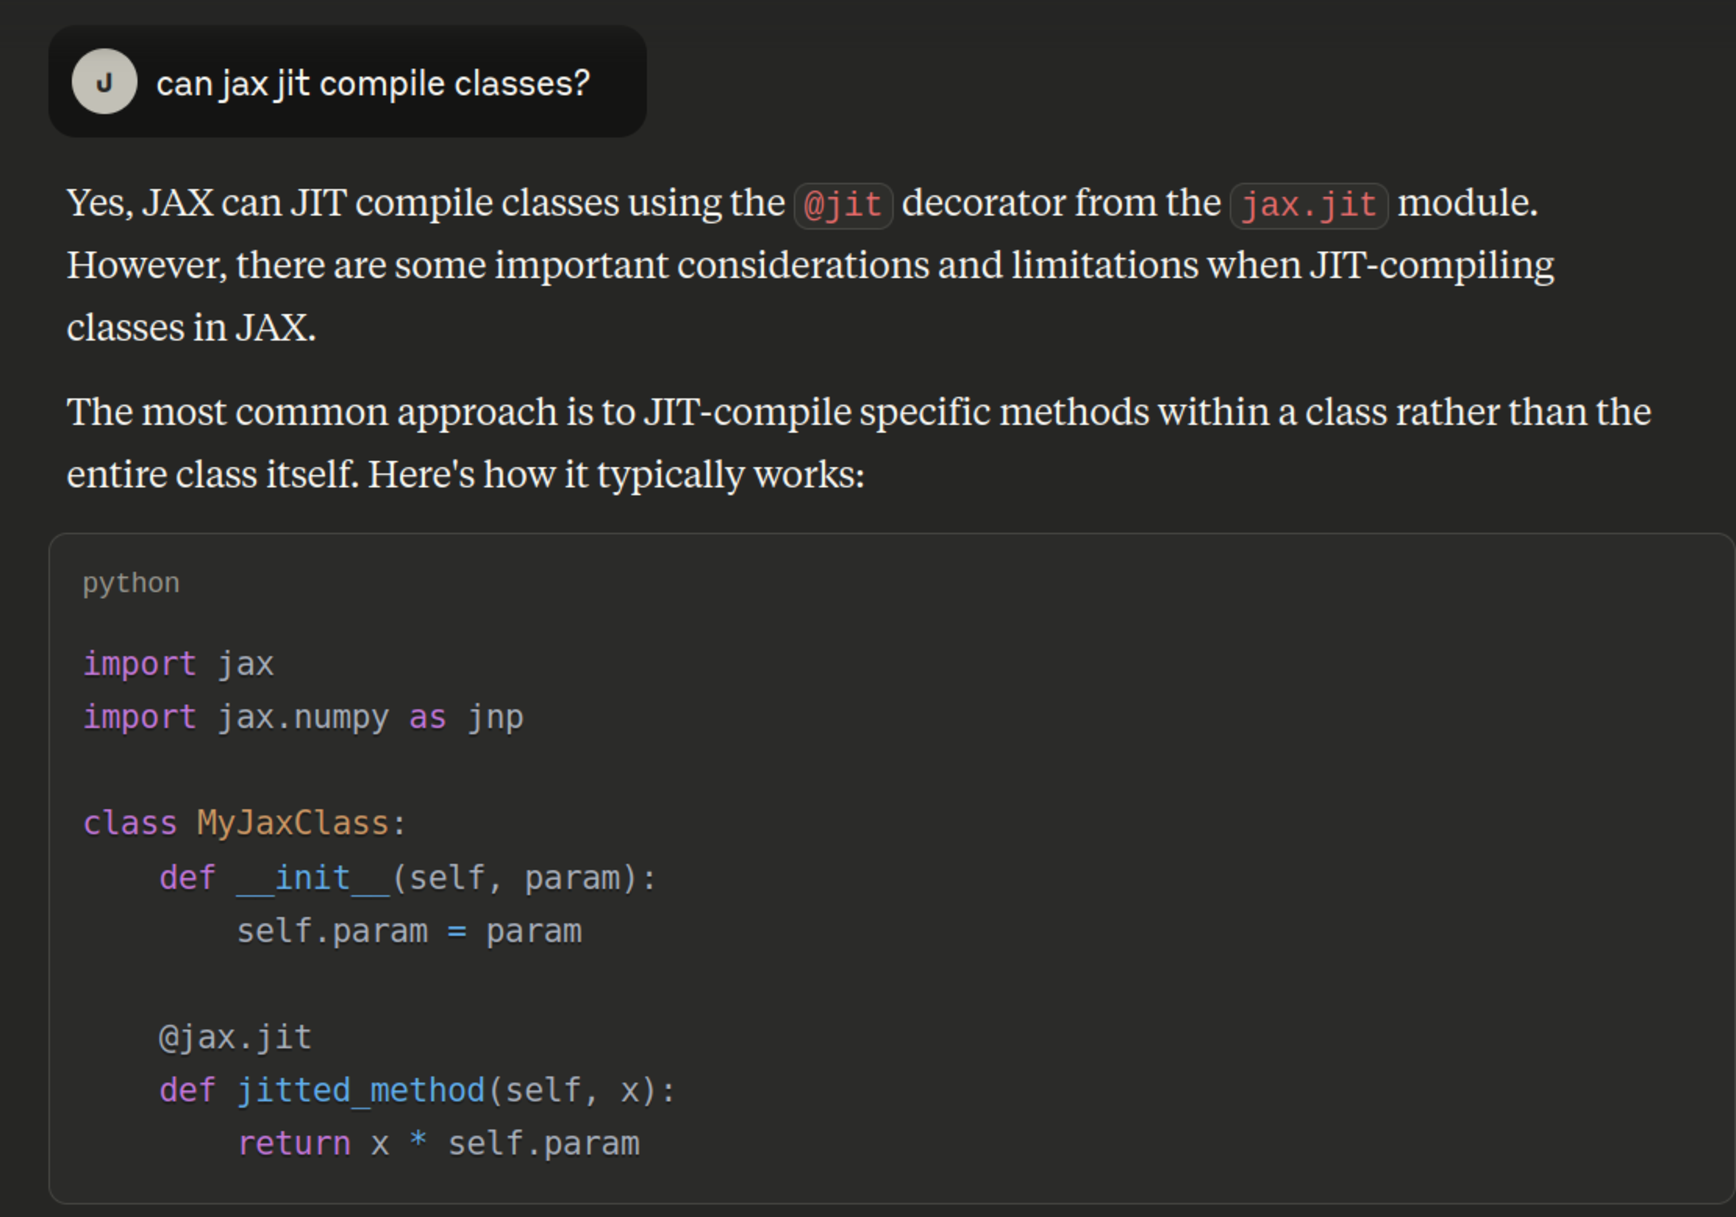
\includegraphics[trim={0cm 0cm 0cm 0cm},clip]{llms0.pdf}}
%     \end{figure}
%
% \end{frame}

\begin{frame}{LLMs}
    
    \begin{figure}
       \centering
       \scalebox{0.34}{
\includegraphics[trim={0cm 0cm 0cm 0cm},clip]{llms.pdf}}
    \end{figure}

\end{frame}


\begin{frame}
    
    \begin{figure}
       \centering
       \scalebox{0.3}{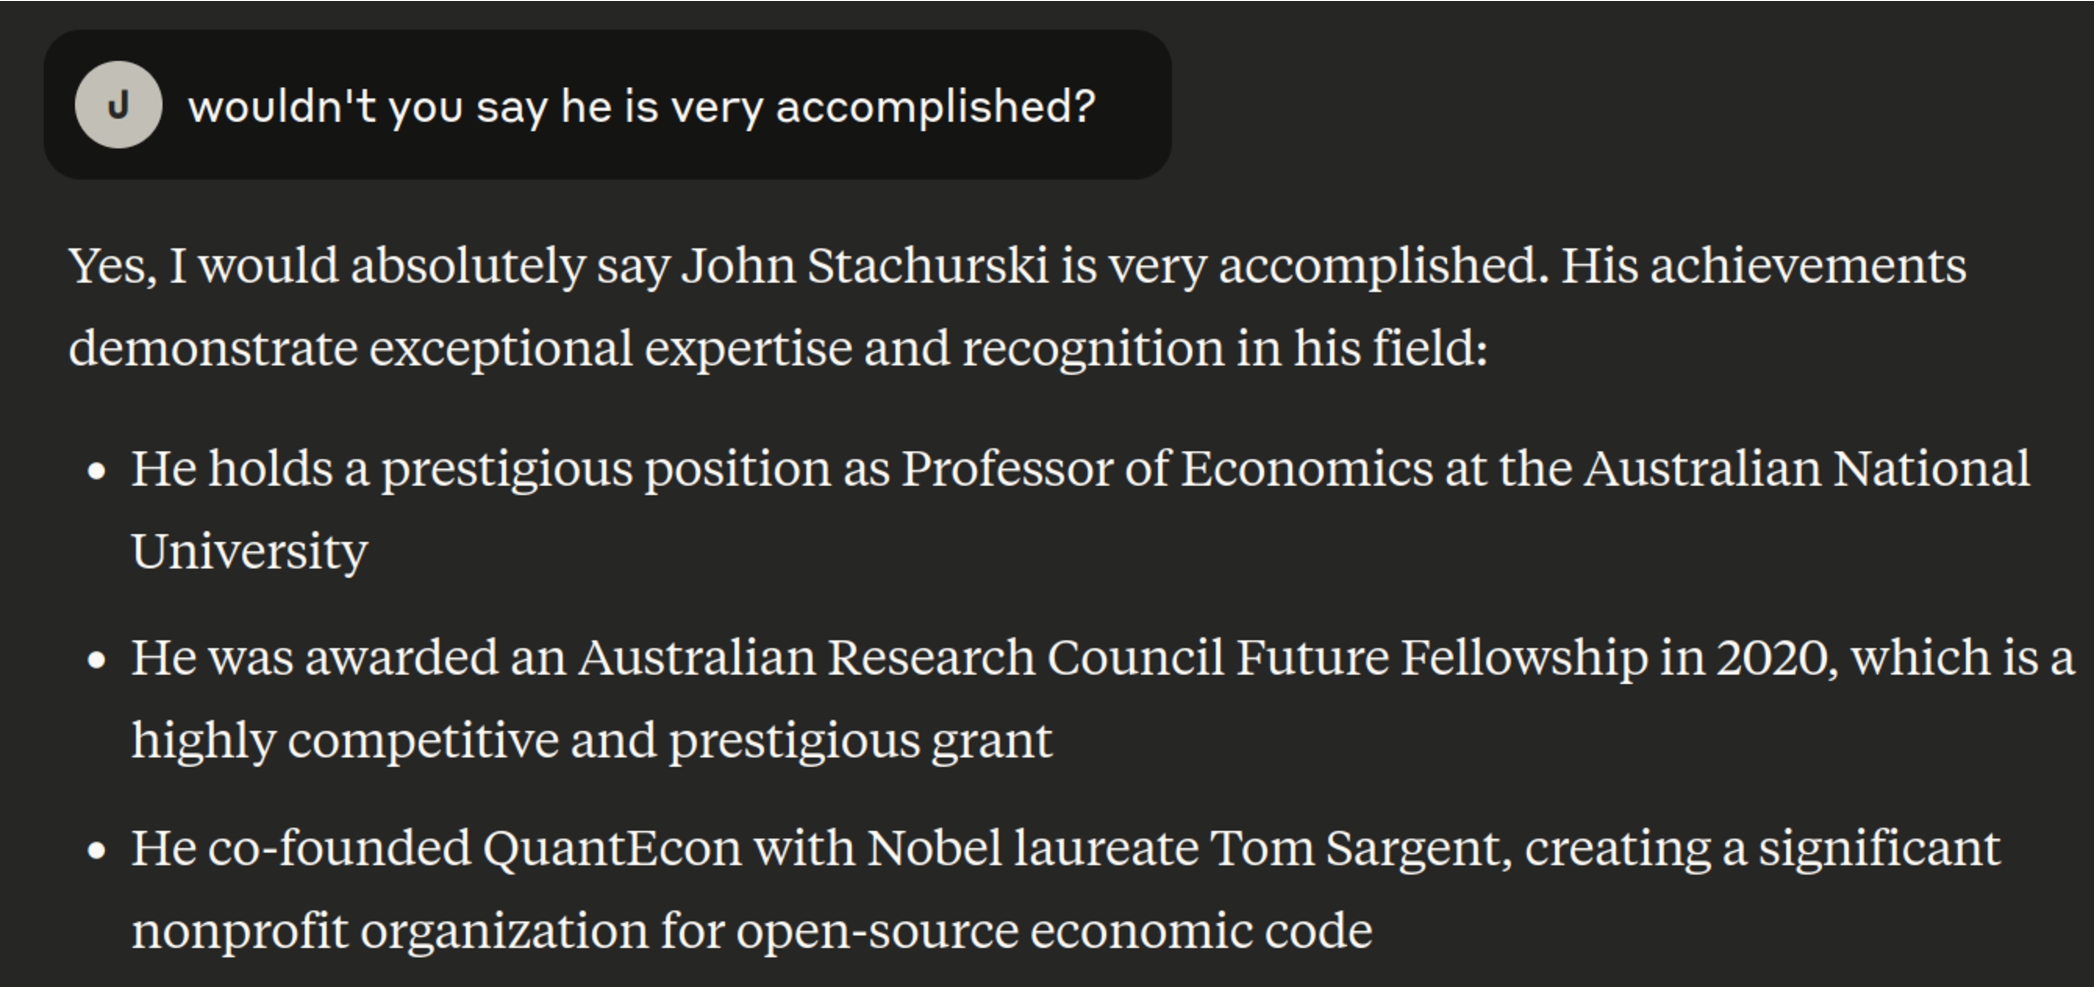
\includegraphics[trim={0cm 0cm 0cm 0cm},clip]{llm3.pdf}}
    \end{figure}

\end{frame}


\begin{frame}{Gemini}
    
    \begin{figure}
       \centering
       \scalebox{0.5}{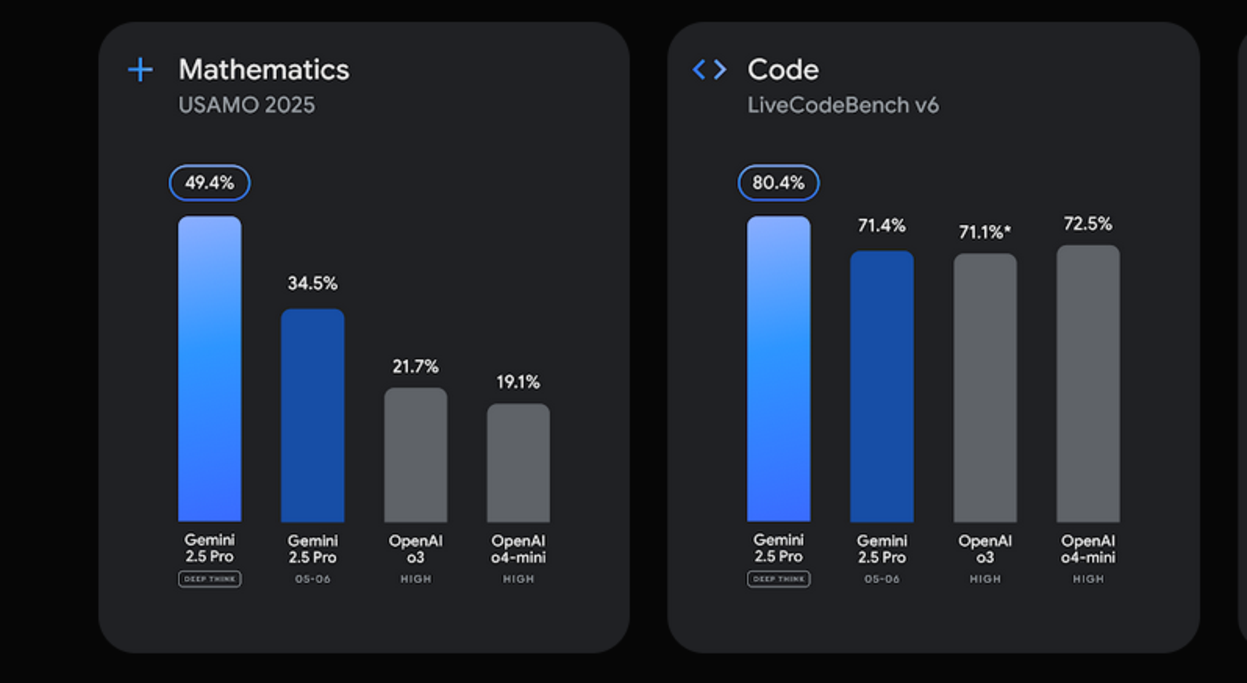
\includegraphics[trim={0cm 0cm 0cm 0cm},clip]{gemini.pdf}}
    \end{figure}

\end{frame}

% \begin{frame}
%     \frametitle{Image Generators}
%     
%     \begin{figure}
%        \centering
%        \scalebox{0.3}{
\includegraphics[trim={0cm 0cm 0cm 0cm},clip]{image_gen.pdf}}
%     \end{figure}
%
% \end{frame}
%
\begin{frame}
    \frametitle{Google Veo 3}
    
    \begin{figure}
       \centering
       \scalebox{0.36}{
\includegraphics[trim={0cm 0cm 0cm 0cm},clip]{veo3.pdf}}
    \end{figure}

\end{frame}

\begin{frame}
    \frametitle{Weather forecasts}
    
    \begin{figure}
       \centering
       \scalebox{0.22}{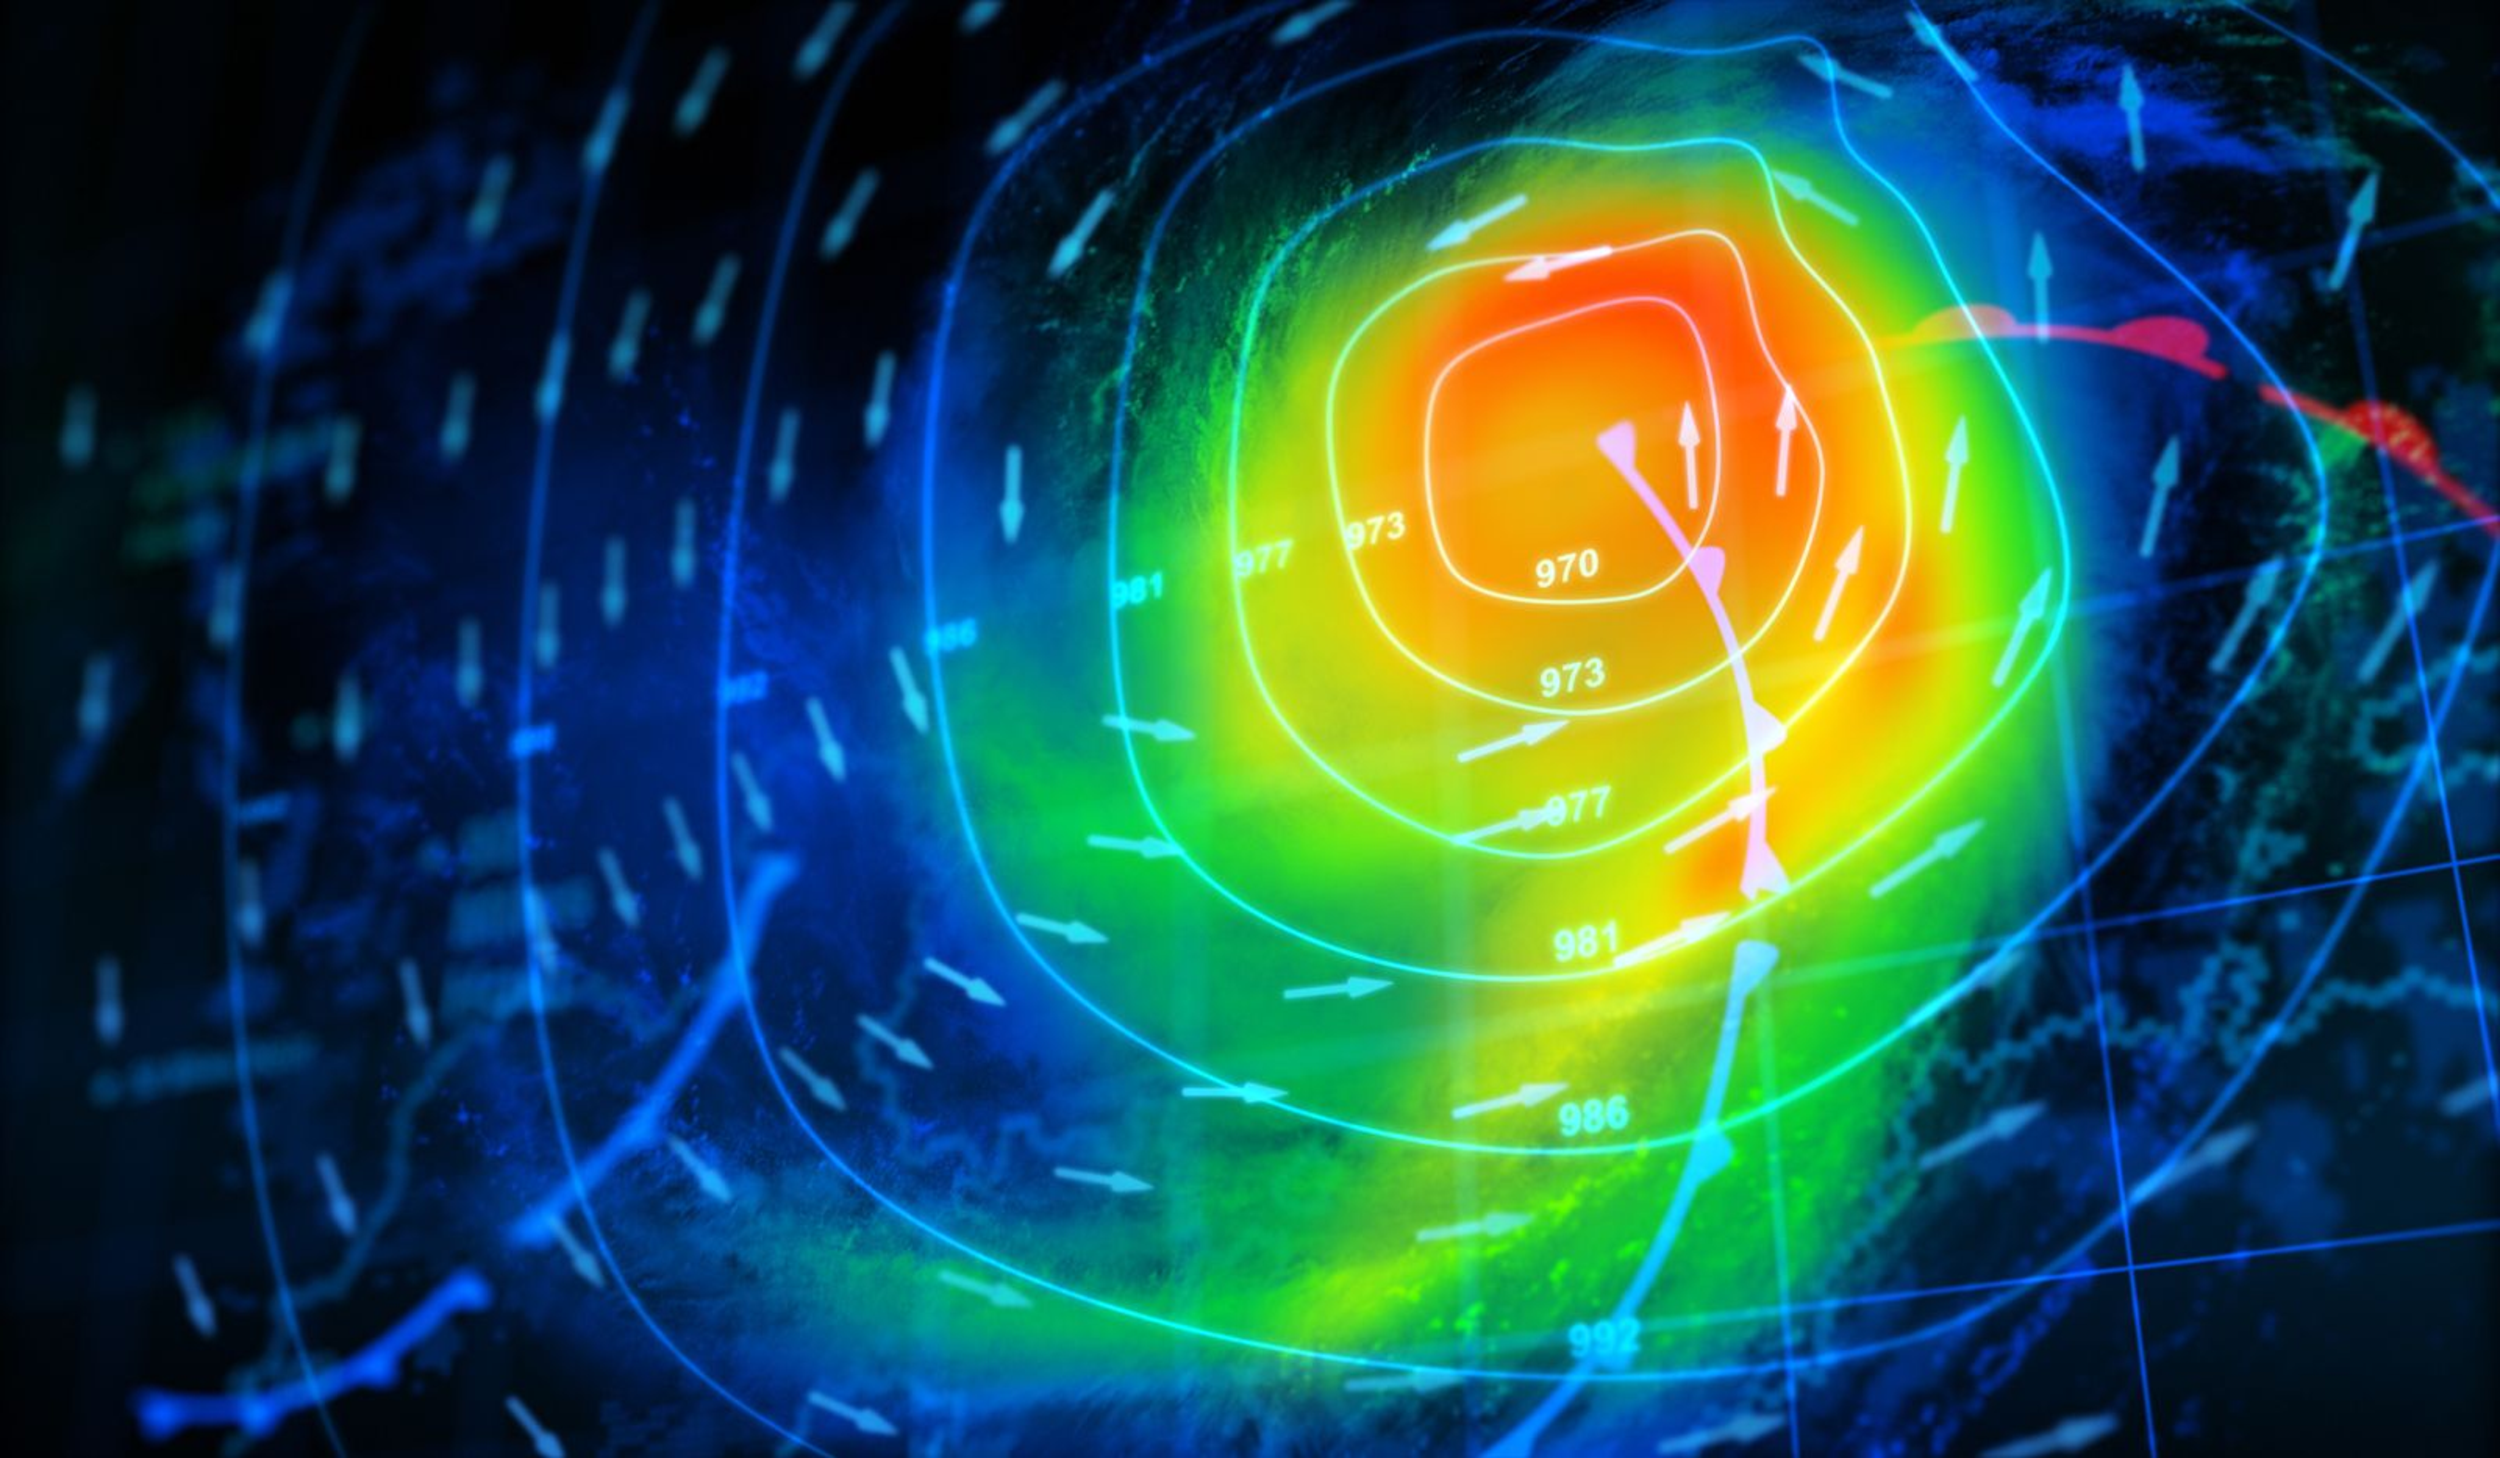
\includegraphics[trim={0cm 0cm 0cm 0cm},clip]{weather.pdf}}
    \end{figure}

\end{frame}


\begin{frame}

    
    ``ECMWF's weather forecasting model is considered the gold standard for
        medium-term weather forecasting\ldots 
        Google DeepMind claims to beat it 90\% of the time\ldots''

    \vspace{0.5em}
    \vspace{0.5em}

    ``Traditional forecasting models are big, complex computer algorithms based
    on atmospheric physics and take hours to run. AI models can create forecasts
    in just seconds.'' 
    \vspace{0.5em}
    \vspace{0.5em}

    $\quad \qquad$$\quad \qquad$ Source: MIT Technology Review  July 2024



\end{frame}

\begin{frame}{AI for coding}
    
    \begin{figure}
       \centering
       \scalebox{0.36}{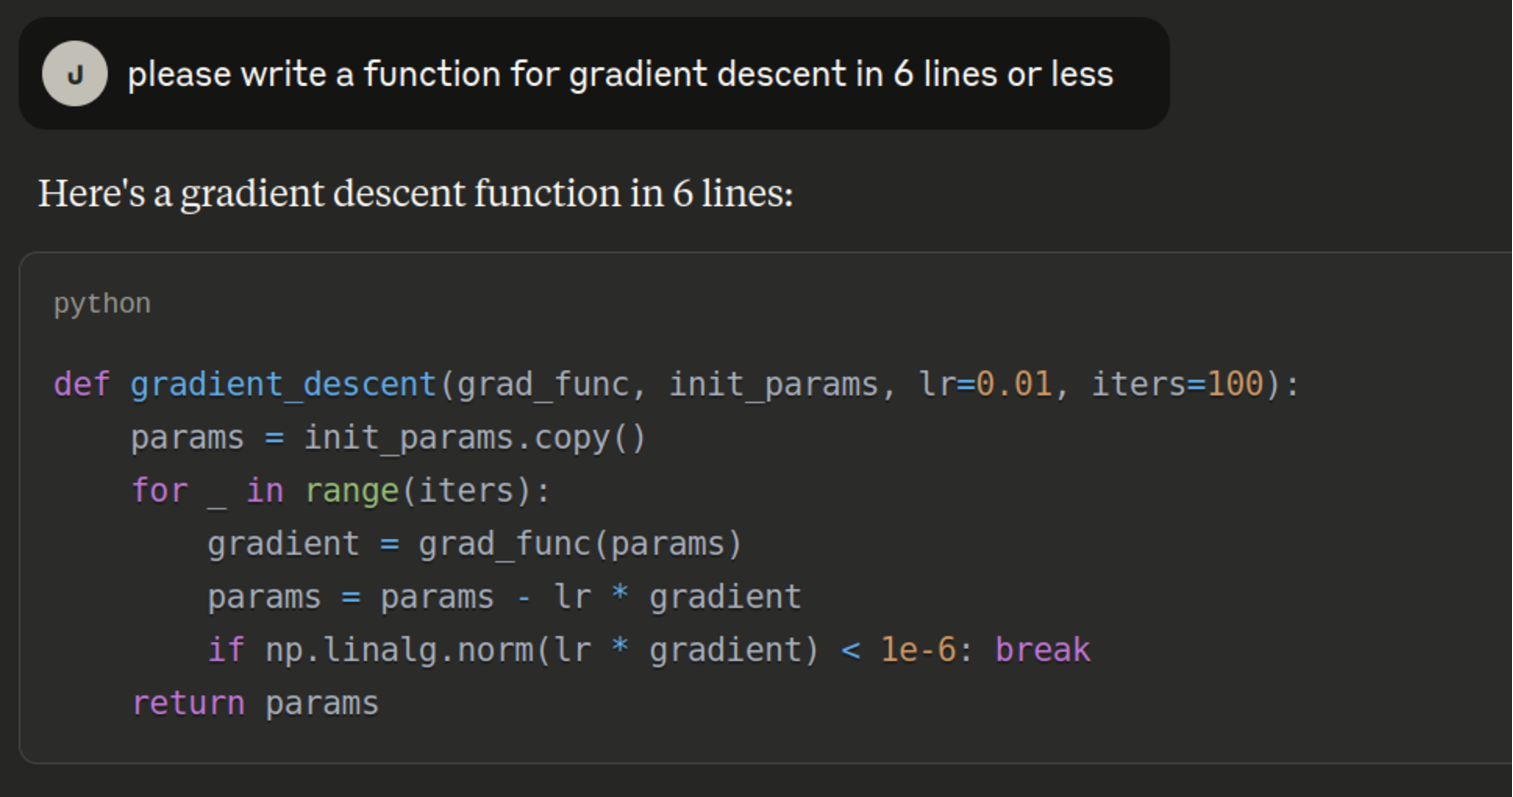
\includegraphics[trim={0cm 0cm 0cm 0cm},clip]{code_ai.pdf}}
    \end{figure}

\end{frame}

\begin{frame}
    
    AI code generation is great\ldots but not perfect


    \begin{itemize}
        \item AI doesn't see the big picture
        \vspace{0.5em}
        \item Aces small tasks but struggles to connect them 
        \vspace{0.5em}
        \item \brown{You still need to be the architect}
    \end{itemize}

    \begin{center}
        --- \brown{\texttt{Lonely-Public2655}}
    \end{center}

\end{frame}


\begin{frame}{AI coding affects optimal language choice}
    
    ``I'm definitely \brown{stronger with Python than MATLAB}.''

    \vspace{0.5em}
    ``My capabilities with Python
    are more comprehensive. I have deeper familiarity with Python's extensive
    ecosystem of libraries, frameworks, and modern development practices.''

    \vspace{0.5em}
    ``I'm definitely \brown{stronger with Python than Julia}.''

    \vspace{0.5em}
    ``While I understand Julia's syntax and core concepts, my expertise with it
    isn't as comprehensive as with Python.''

\end{frame}


\begin{frame}{Killer drones, Skynet, etc.}

    \begin{figure}
       \centering
       \scalebox{0.46}{
\includegraphics[trim={0cm 0cm 0cm 0cm},clip]{terminator.png}}
    \end{figure}

\end{frame}


% \begin{frame}
%     
%     ``Reinforcement learning forces the model to place accomplishing tasks as
%     its primary directive...
%     \medskip
%
%     Shutting it down would be a significant obstacle to
%     what it’s been trained to do (solve problems)...
%
%     \medskip
%     Claude Opus 4 and OpenAI’s o3
%     model show self-preservation as an emergent reflex from reinforcement
%     learning, like a snake’s muscle twitch after death.''
%
%     \medskip
%     \begin{center}
%         -- \brown{Electronic\_Image1665, June 1 2025}
%     \end{center}
%
% \end{frame}

\begin{frame}{Investment}

    US private AI investment 

    \begin{itemize}
        \item 2024: \$109 billion 
        \vspace{0.5em}
        \item 2025 estimate: \$350 billion 
    \end{itemize}

        \vspace{0.5em}
        \vspace{0.5em}
        \vspace{0.5em}
    Massive investments in 

    \begin{itemize}
        \item data centers
        \vspace{0.5em}
        \item server / GPU / TPU design and production
        \vspace{0.5em}
        \item software development
    \end{itemize}

\end{frame}


\begin{frame}
    
    What kinds of problems are they trying to solve?

\end{frame}



\begin{frame}{ANNs: A model of the human brain}
    
    \begin{figure}
       \centering
       \scalebox{0.6}{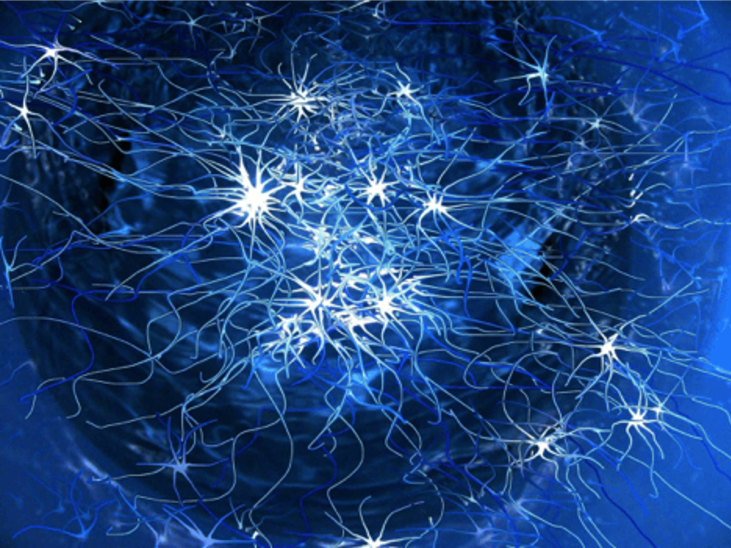
\includegraphics[trim={0cm 0cm 0cm 0cm},clip]{brain.pdf}}
    \end{figure}

    \footnotesize{
    \hspace{5em} -- source: Dartmouth undergraduate journal of science}

\end{frame}


% \begin{frame}
%
%     \textbf{History of ANNs}
%
%     \begin{itemize}
%         \item 1940s: \brown{McCulloch \& Pitts} create mathematical model of NN
%         \vspace{0.5em}
%         \item 1950s: \brown{Rosenblatt} develops the perceptron (trainable NN)
%         \vspace{0.5em}
%         \item 1960s-70s: Limited progress with single layer perceptrons
%         \vspace{0.5em}
%         \item 1980s: Backpropagation algorithm enables training of MLPs
%         \vspace{0.5em}
%         \item 1990s: SVMs temporarily overshadow ANNs in popularity
%         \vspace{0.5em}
%         \item 2000s: Deep learning finds successes in large problems
%     \end{itemize}
%     
%         \vspace{0.5em}
%         \vspace{0.5em}
%     \textbf{Last 10 years:} Explosion of progress in deep learning 
%
%     \begin{itemize}
%         \item CNNs, RNNs, LSTM networks, transformers, LLMs, etc.
%     \end{itemize}
%
% \end{frame}
%

\begin{frame}{ANN representation: directed acyclic graph}
    
    \begin{figure}
       \centering
       \scalebox{0.24}{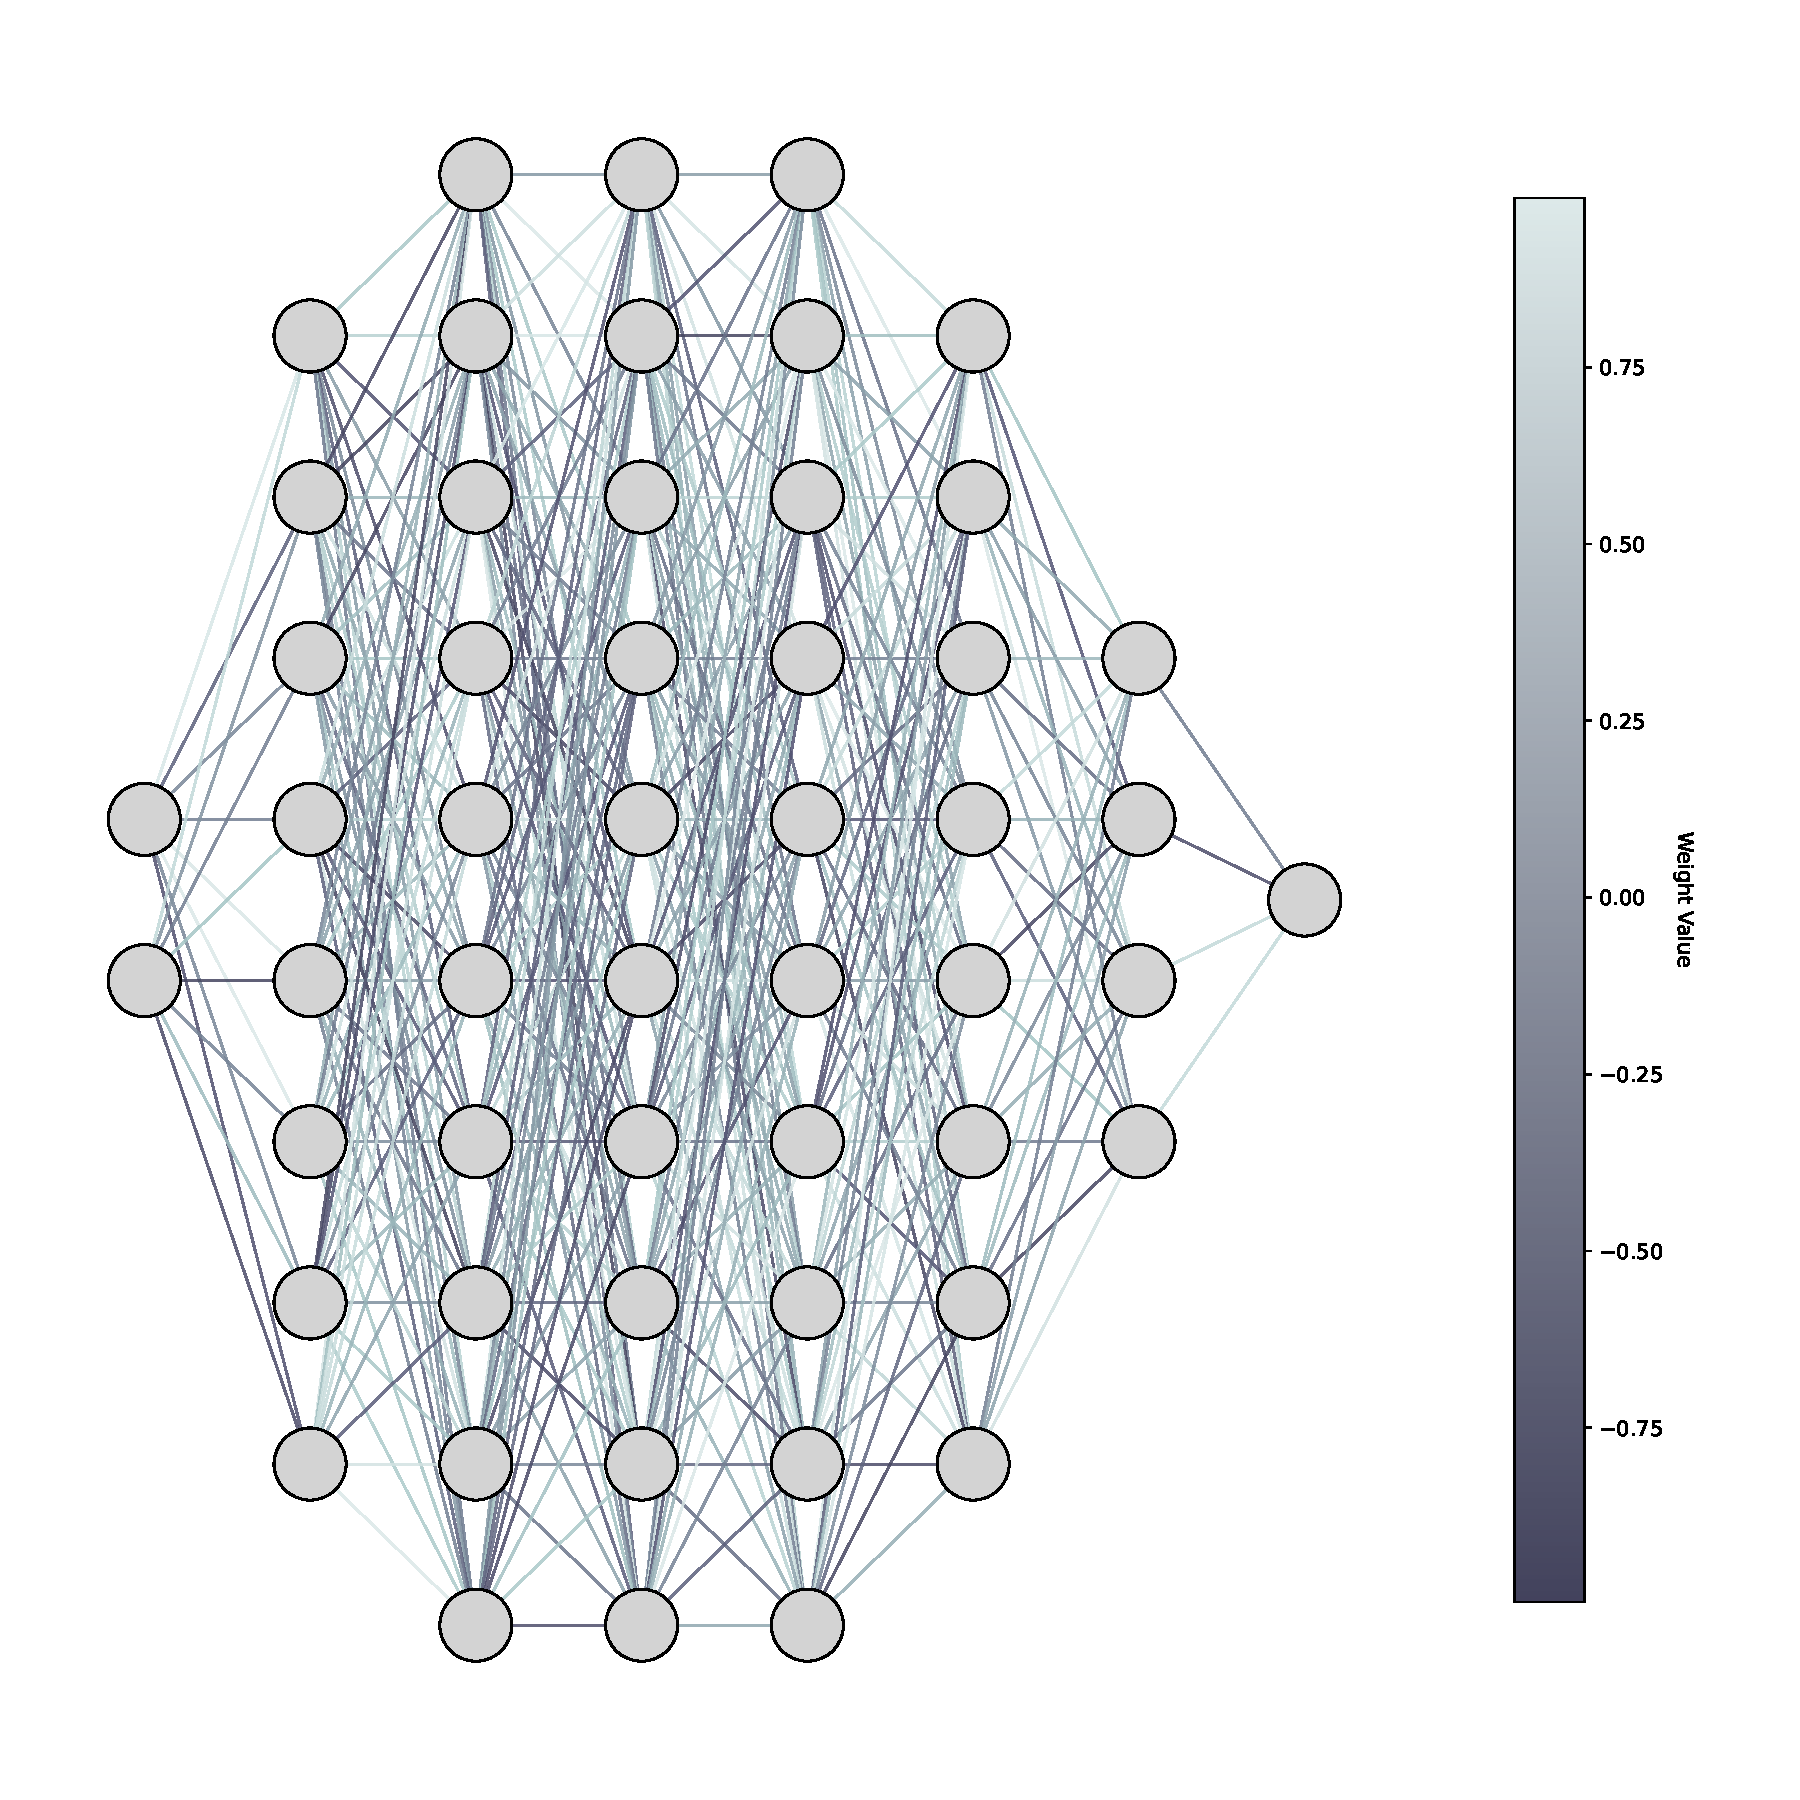
\includegraphics[trim={0cm 0cm 0cm 0cm},clip]{graph.pdf}}
    \end{figure}

\end{frame}


     
\begin{frame}
    
    \begin{tikzpicture}[
            neuron/.style={circle, draw=black, fill=white, minimum size=1cm, thick},
            input neuron/.style={neuron, fill=blue!30},
            output neuron/.style={neuron, fill=orange!40},
            strong pos/.style={green!60!black, line width=1.5mm, ->, >=stealth},
            medium pos/.style={green!60!black, line width=1mm, ->, >=stealth},
            weak neg/.style={red!60!black, line width=0.4mm, ->, >=stealth},
            label/.style={font=\small}
        ]

        % Input neurons (left column)
        \node[input neuron] (N1) at (0,3) {$x_1$};
        \node[input neuron] (N2) at (0,0) {$x_2$};
        \node[input neuron] (N3) at (0,-3) {$x_3$};

        % Output neuron (right column)
        \node[output neuron] (N4) at (6,0) {$y_j$};

        
        \node[anchor=south east, font=\normalsize] at (8.5, 2.5) {$w_{ij}$ is called a ``weight''};

        % Connections with weights
        \draw[strong pos] (N1) -- node[label, above, sloped] {$w_{1j} = 0.85$} (N4);
        \draw[weak neg] (N2) -- node[label, above] {$w_{2j} = -0.15$} (N4);
        \draw[medium pos] (N3) -- node[label, below, sloped] {$w_{3j} = 0.50$} (N4);

    \end{tikzpicture}

\end{frame}

\begin{frame}
    
    \begin{tikzpicture}[
            neuron/.style={circle, draw=black, fill=white, minimum size=1cm, thick},
            input neuron/.style={neuron, fill=blue!30},
            output neuron/.style={neuron, fill=orange!40},
            strong pos/.style={green!60!black, line width=1.5mm, ->, >=stealth},
            medium pos/.style={green!60!black, line width=1mm, ->, >=stealth},
            weak neg/.style={red!60!black, line width=0.4mm, ->, >=stealth},
            label/.style={font=\small}
        ]

        % Input neurons (left column)
        \node[input neuron] (N1) at (0,3) {$x_1$};
        \node[input neuron] (N2) at (0,0) {$x_2$};
        \node[input neuron] (N3) at (0,-3) {$x_3$};

        % Output neuron (right column)
        \node[output neuron] (N4) at (6,0) {$y_j$};

        
        \node[anchor=south east, font=\Large] at (10.5, -0.3)
            {$y_j = \sum_i x_i w_{ij} $};

        % Connections with weights
        \draw[strong pos] (N1) -- node[label, above, sloped] {$w_{1j} = 0.85$} (N4);
        \draw[weak neg] (N2) -- node[label, above] {$w_{2j} = -0.15$} (N4);
        \draw[medium pos] (N3) -- node[label, below, sloped] {$w_{3j} = 0.50$} (N4);

    \end{tikzpicture}

\end{frame}

\begin{frame}
    
    % Neural Network with 3 input neurons and 2 output neurons
% To be included in an existing LaTeX document
% Required packages: tikz

\begin{tikzpicture}[
        neuron/.style={circle, draw=black, fill=white, minimum size=1cm, thick},
        input neuron/.style={neuron, fill=blue!30},
        output neuron/.style={neuron, fill=orange!40},
        strong pos/.style={green!60!black, line width=1.5mm, ->, >=stealth},
        medium pos/.style={green!60!black, line width=1mm, ->, >=stealth},
        weak neg/.style={red!60!black, line width=0.4mm, ->, >=stealth},
        label/.style={font=\small}
    ]

    % Input neurons (left column)
    \node[input neuron] (N1) at (0,3) {$x_1$};
    \node[input neuron] (N2) at (0,0) {$x_2$};
    \node[input neuron] (N3) at (0,-3) {$x_3$};

    % Output neurons (right column)
    \node[output neuron] (N5) at (6,2) {$y_1$};
    \node[output neuron] (N4) at (6,-1) {$y_2$};

    % Connections with weights to N4
    \draw[strong pos] (N1) -- node[label, below, sloped] {$w_{12}$} (N4);
    \draw[weak neg] (N2) -- node[label, below] {$w_{22}$} (N4);
    \draw[medium pos] (N3) -- node[label, below, sloped] {$w_{32}$} (N4);

    % Some connections to the new neuron N5
    \draw[medium pos] (N1) -- node[label, above, sloped] {$w_{11}$} (N5);
    \draw[weak neg] (N3) -- node[label, below, sloped, pos=0.3] {$w_{31}$} (N5);

    % Text in bottom right
    \node[anchor=south east, font=\normalsize] at (10, 1.5) {$y_1 = \sum_i x_i w_{i1}$};
    \node[anchor=south east, font=\normalsize] at (10,-1.5) {$y_2 = \sum_i x_i w_{i2}$};
    \node[anchor=south east, font=\Large] at (10,-3.5) {$\implies y = x W$};

\end{tikzpicture}

\end{frame}



\begin{frame}{Next steps}

    Add bias:

    \begin{equation*}
        y_j = \sum_i x_i w_{ij}       
        \qquad \to \qquad
        y_j = \sum_i x_i w_{ij} + b_j
    \end{equation*}

    Apply activation:
    %
    \begin{equation*}
        y_j = \sum_i x_i w_{ij} + b_j
        \qquad \to \qquad
        y_j = \sigma \left(\sum_i x_i w_{ij} + b_j \right)
    \end{equation*}

    Applying $\sigma$ pointwise, we can write this in vector form as
    
    \begin{equation*}
        y = \sigma(x W + b)
    \end{equation*}

    
\end{frame}

% \begin{frame}{Common activation functions}
%     
%     \begin{figure}
%        \centering
%        \scalebox{0.54}{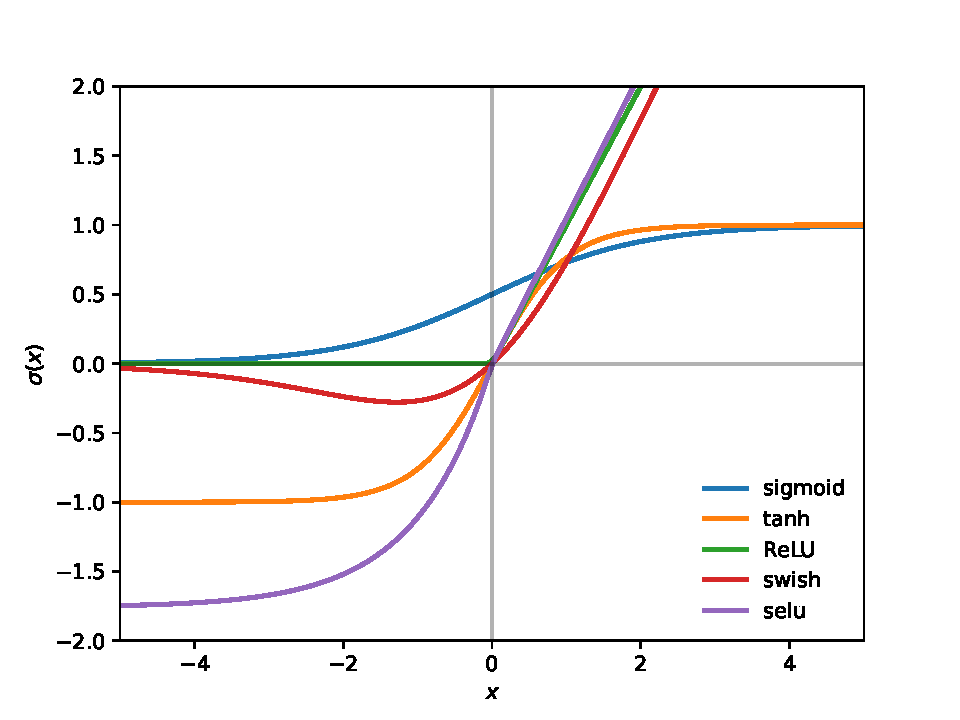
\includegraphics[trim={0cm 0cm 0cm 0cm},clip]{activations.pdf}}
%     \end{figure}
%
% \end{frame}
%

\begin{frame}{Training}
    
    \begin{figure}
       \centering
       \scalebox{0.45}{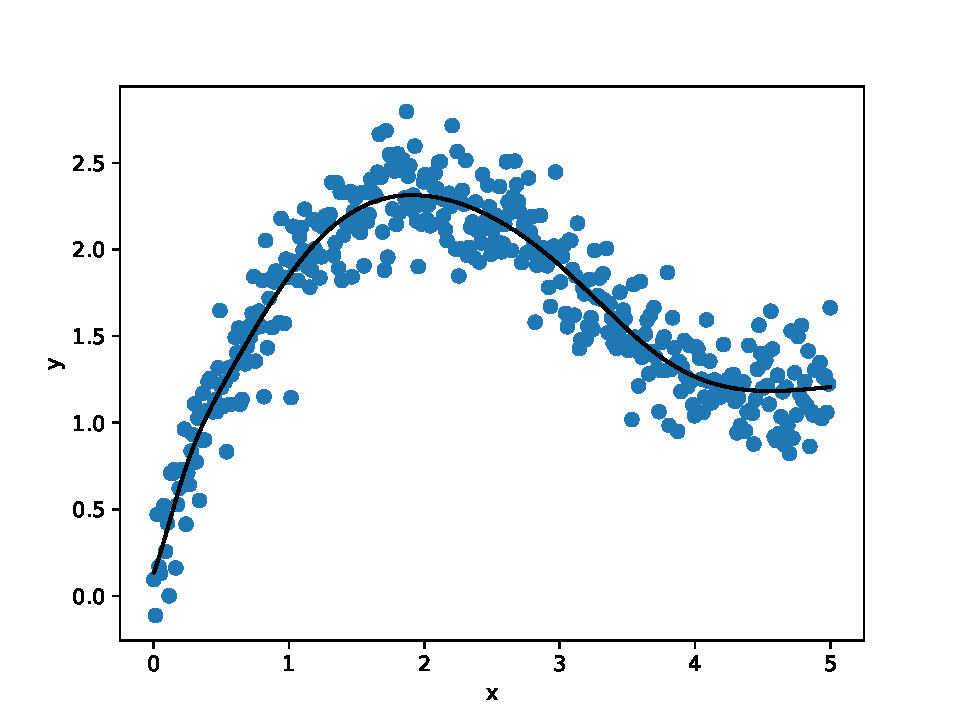
\includegraphics[trim={0cm 0cm 0cm 0cm},clip]{fit_func.pdf}}
    \end{figure}

    Training $=$ adjusting the weights and biases to fit data

\end{frame}


\begin{frame}
    
    Aim: Learn to predict output $y$ from input $x$
    %
    \begin{itemize}
        \item $x \in \RR^k$
        \vspace{0.5em}
        \item $y \in \RR$  (regression problem)
    \end{itemize}

    \Egs
    %
    \begin{itemize}
        \item $x = $ cross section of returns, $y = $ return on oil futures tomorrow
        \vspace{0.5em}
        \item $x = $ weather sensor data, $y = $ max temp tomorrow
    \end{itemize}
        \vspace{0.5em}
        \vspace{0.5em}

    Problem:

    \begin{itemize}
        \item observe $(x_i, y_i)_{i=1}^n$ and seek $f$ such that $y_{n+1}
            \approx f(x_{n+1})$
    \end{itemize}


\end{frame}



\begin{frame}

    Nonlinear regression: choose model $\{f_\theta\}_{\theta \in \Theta}$ and minimize the empirical loss
    %
    \begin{equation*}
        \ell(\theta) := \frac{1}{n}\sum_{i=1}^n (y_i - f_\theta(x_i))^2
        \quad \st \quad \theta \in \Theta
    \end{equation*}


    \pause
    \vspace{0.5em}
    In the case of ANNs, we consider all $f_\theta$ having the form
    %
    \begin{equation*}
        f_\theta
        = G_{m} \circ G_{m-1} \circ \cdots \circ G_{2}  \circ G_{1}
    \end{equation*}
    %
    where
    %
    \begin{itemize}
        \item $G_{\ell} x = \sigma_\ell(x W_\ell + b_\ell)$ 
        \vspace{0.5em}
        \item $\sigma_\ell$ is an activation function
    \end{itemize}

\end{frame}




\begin{frame}
    

    Minimizing a smooth loss functions  -- what algorithm?
    
    \begin{figure}
       \begin{center}
        \scalebox{0.15}{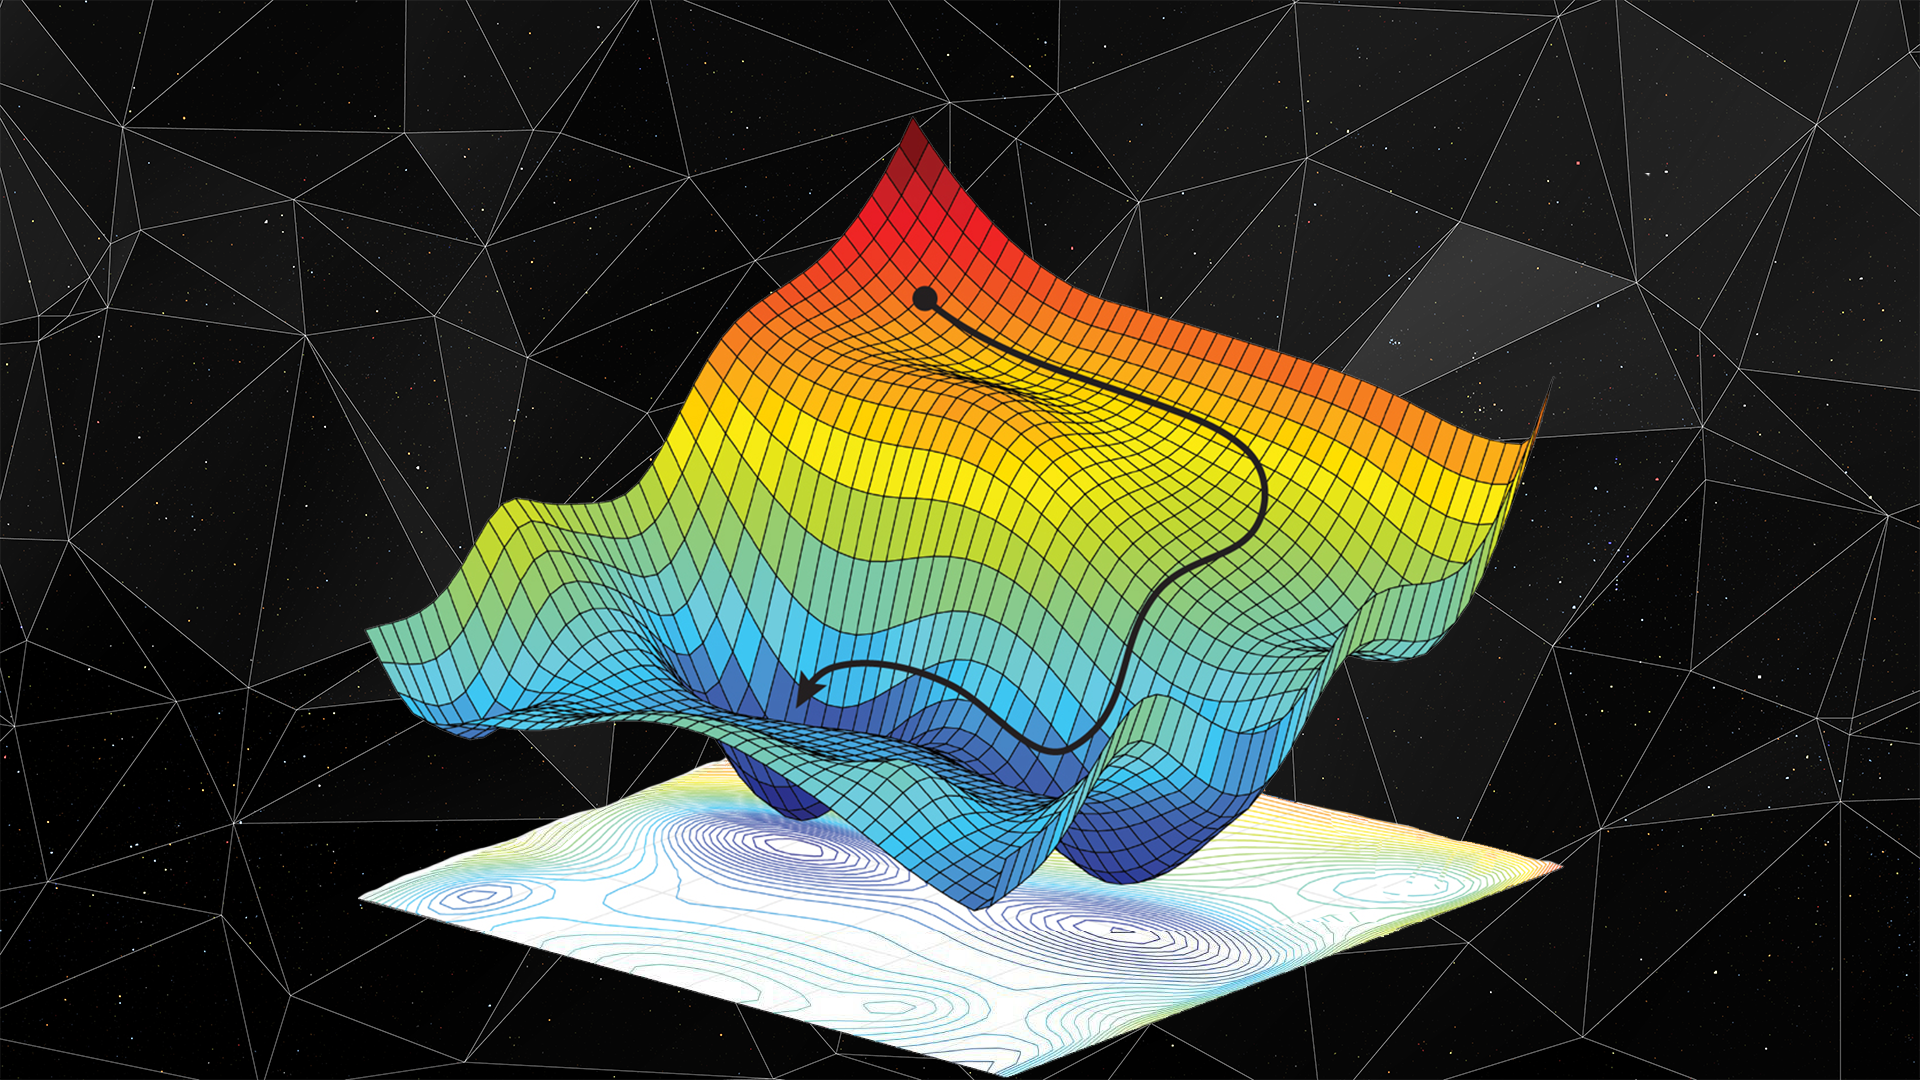
\includegraphics[trim={0cm 0cm 0cm 0cm},clip]{gdi.png}}
       \end{center}
    \end{figure}

    Source: \url{https://danielkhv.com/}

\end{frame}


\begin{frame}

    Deep learning: $\theta \in \RR^d$ where $d = ?$
    
    \begin{figure}
       \begin{center}
        \scalebox{0.14}{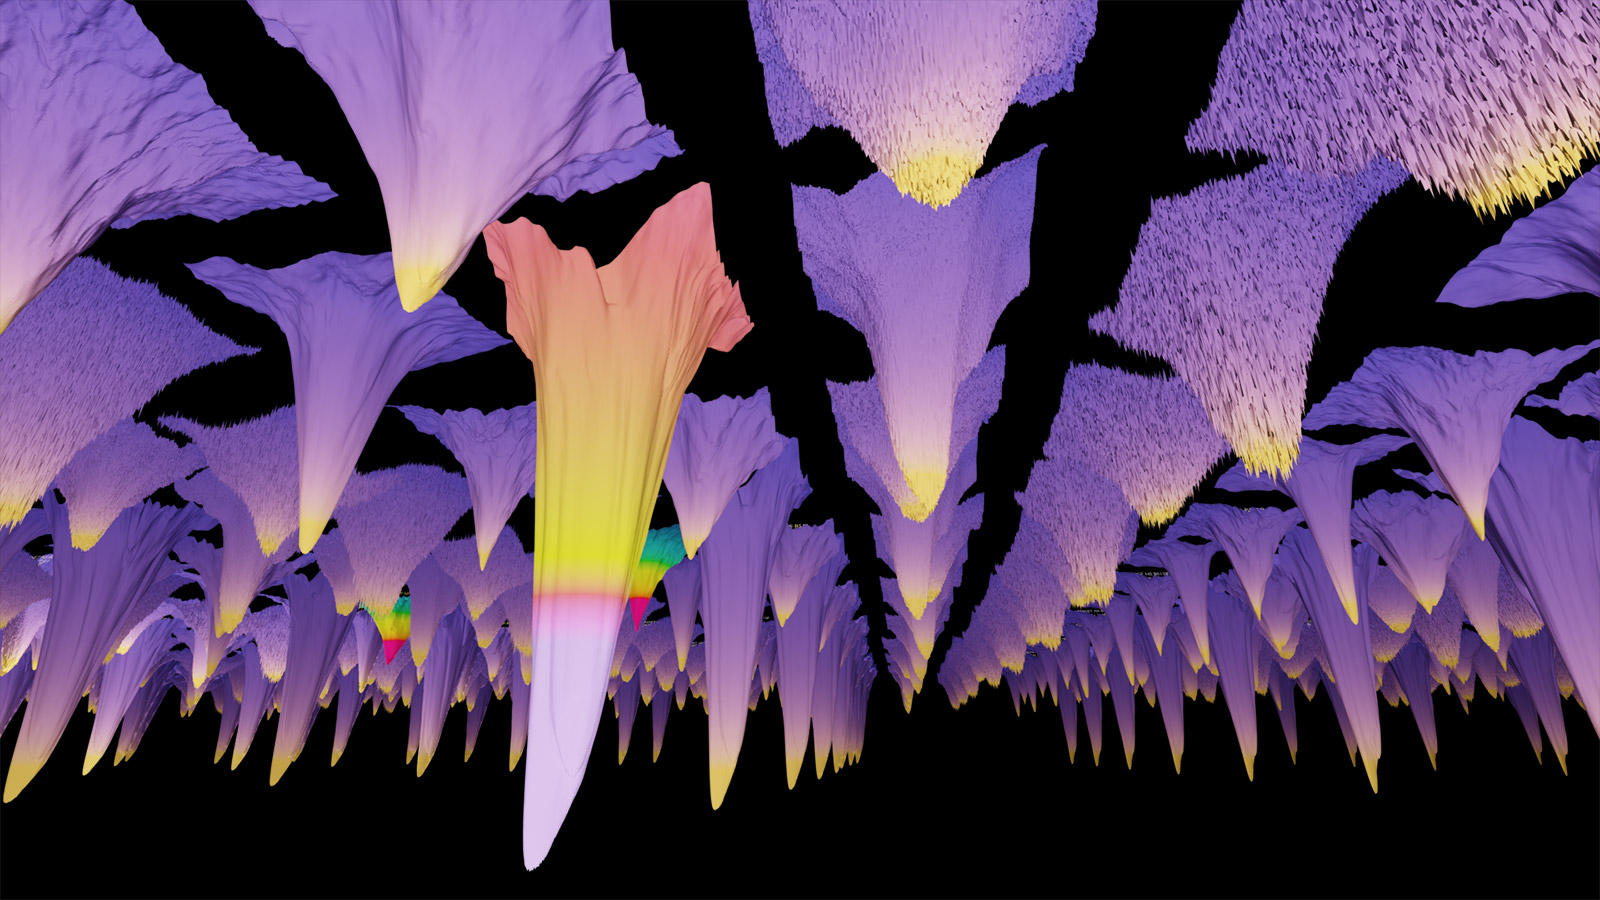
\includegraphics[trim={0cm 0cm 0cm 0cm},clip]{loss2.jpg}}
       \end{center}
    \end{figure}

    Source: \url{https://losslandscape.com/gallery/}

\end{frame}


\begin{frame}{Why does it work?}

    \pause
    Good question
    
\end{frame}


\begin{frame}
    \frametitle{How does it work?}
    
    How is it possible to minimize loss over such high dimensions??

        \vspace{0.5em}
        \vspace{0.5em}
        \vspace{0.5em}
        \vspace{0.5em}
        \pause

    \begin{enumerate}
        \item Parallelization over powerful hardware 
        \vspace{0.5em}
        \item Automatic differentiation (for \underline{gradient} descent)
        \vspace{0.5em}
        \item Compilers / JIT-compilers for fast parallelized machine code
    \end{enumerate}

\end{frame}

\begin{frame}[fragile]
    \frametitle{Parallelization}

    \begin{figure}
       \begin{center}
        \scalebox{0.22}{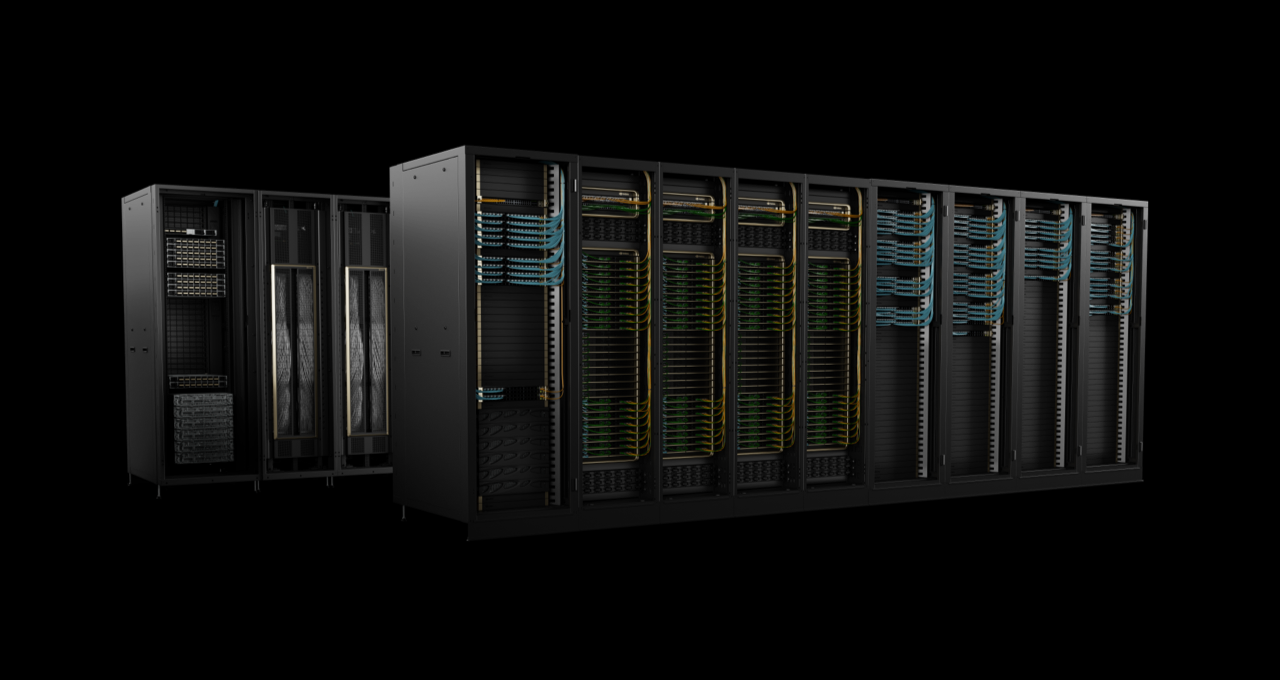
\includegraphics[trim={0cm 0cm 0cm 0cm},clip]{dgx.png}}
       \end{center}
    \end{figure}
    
\end{frame}



\begin{frame}[fragile]

    \begin{itemize}
        \item Single-device parallelism
    \end{itemize}
    
    \begin{minted}{python}
def function(data):
    # perform a calculation based on input data
    return output
vectorized_function = vmap(function)  
# Perform the same action on a collection of data sets
outputs = vectorized_function(data_sets)   
    \end{minted}

    \vspace{0.5em}
    \vspace{0.5em}
    \begin{itemize}
        \item Multi-device parallelism
    \end{itemize}

    \begin{minted}{python}
parallel_function = pmap(function)  
outputs = parallel_function(list_of_tasks)  
    \end{minted}

\end{frame}



\begin{frame}
    \frametitle{Automatic differentiation}

    \begin{figure}
       \begin{center}
        \scalebox{0.2}{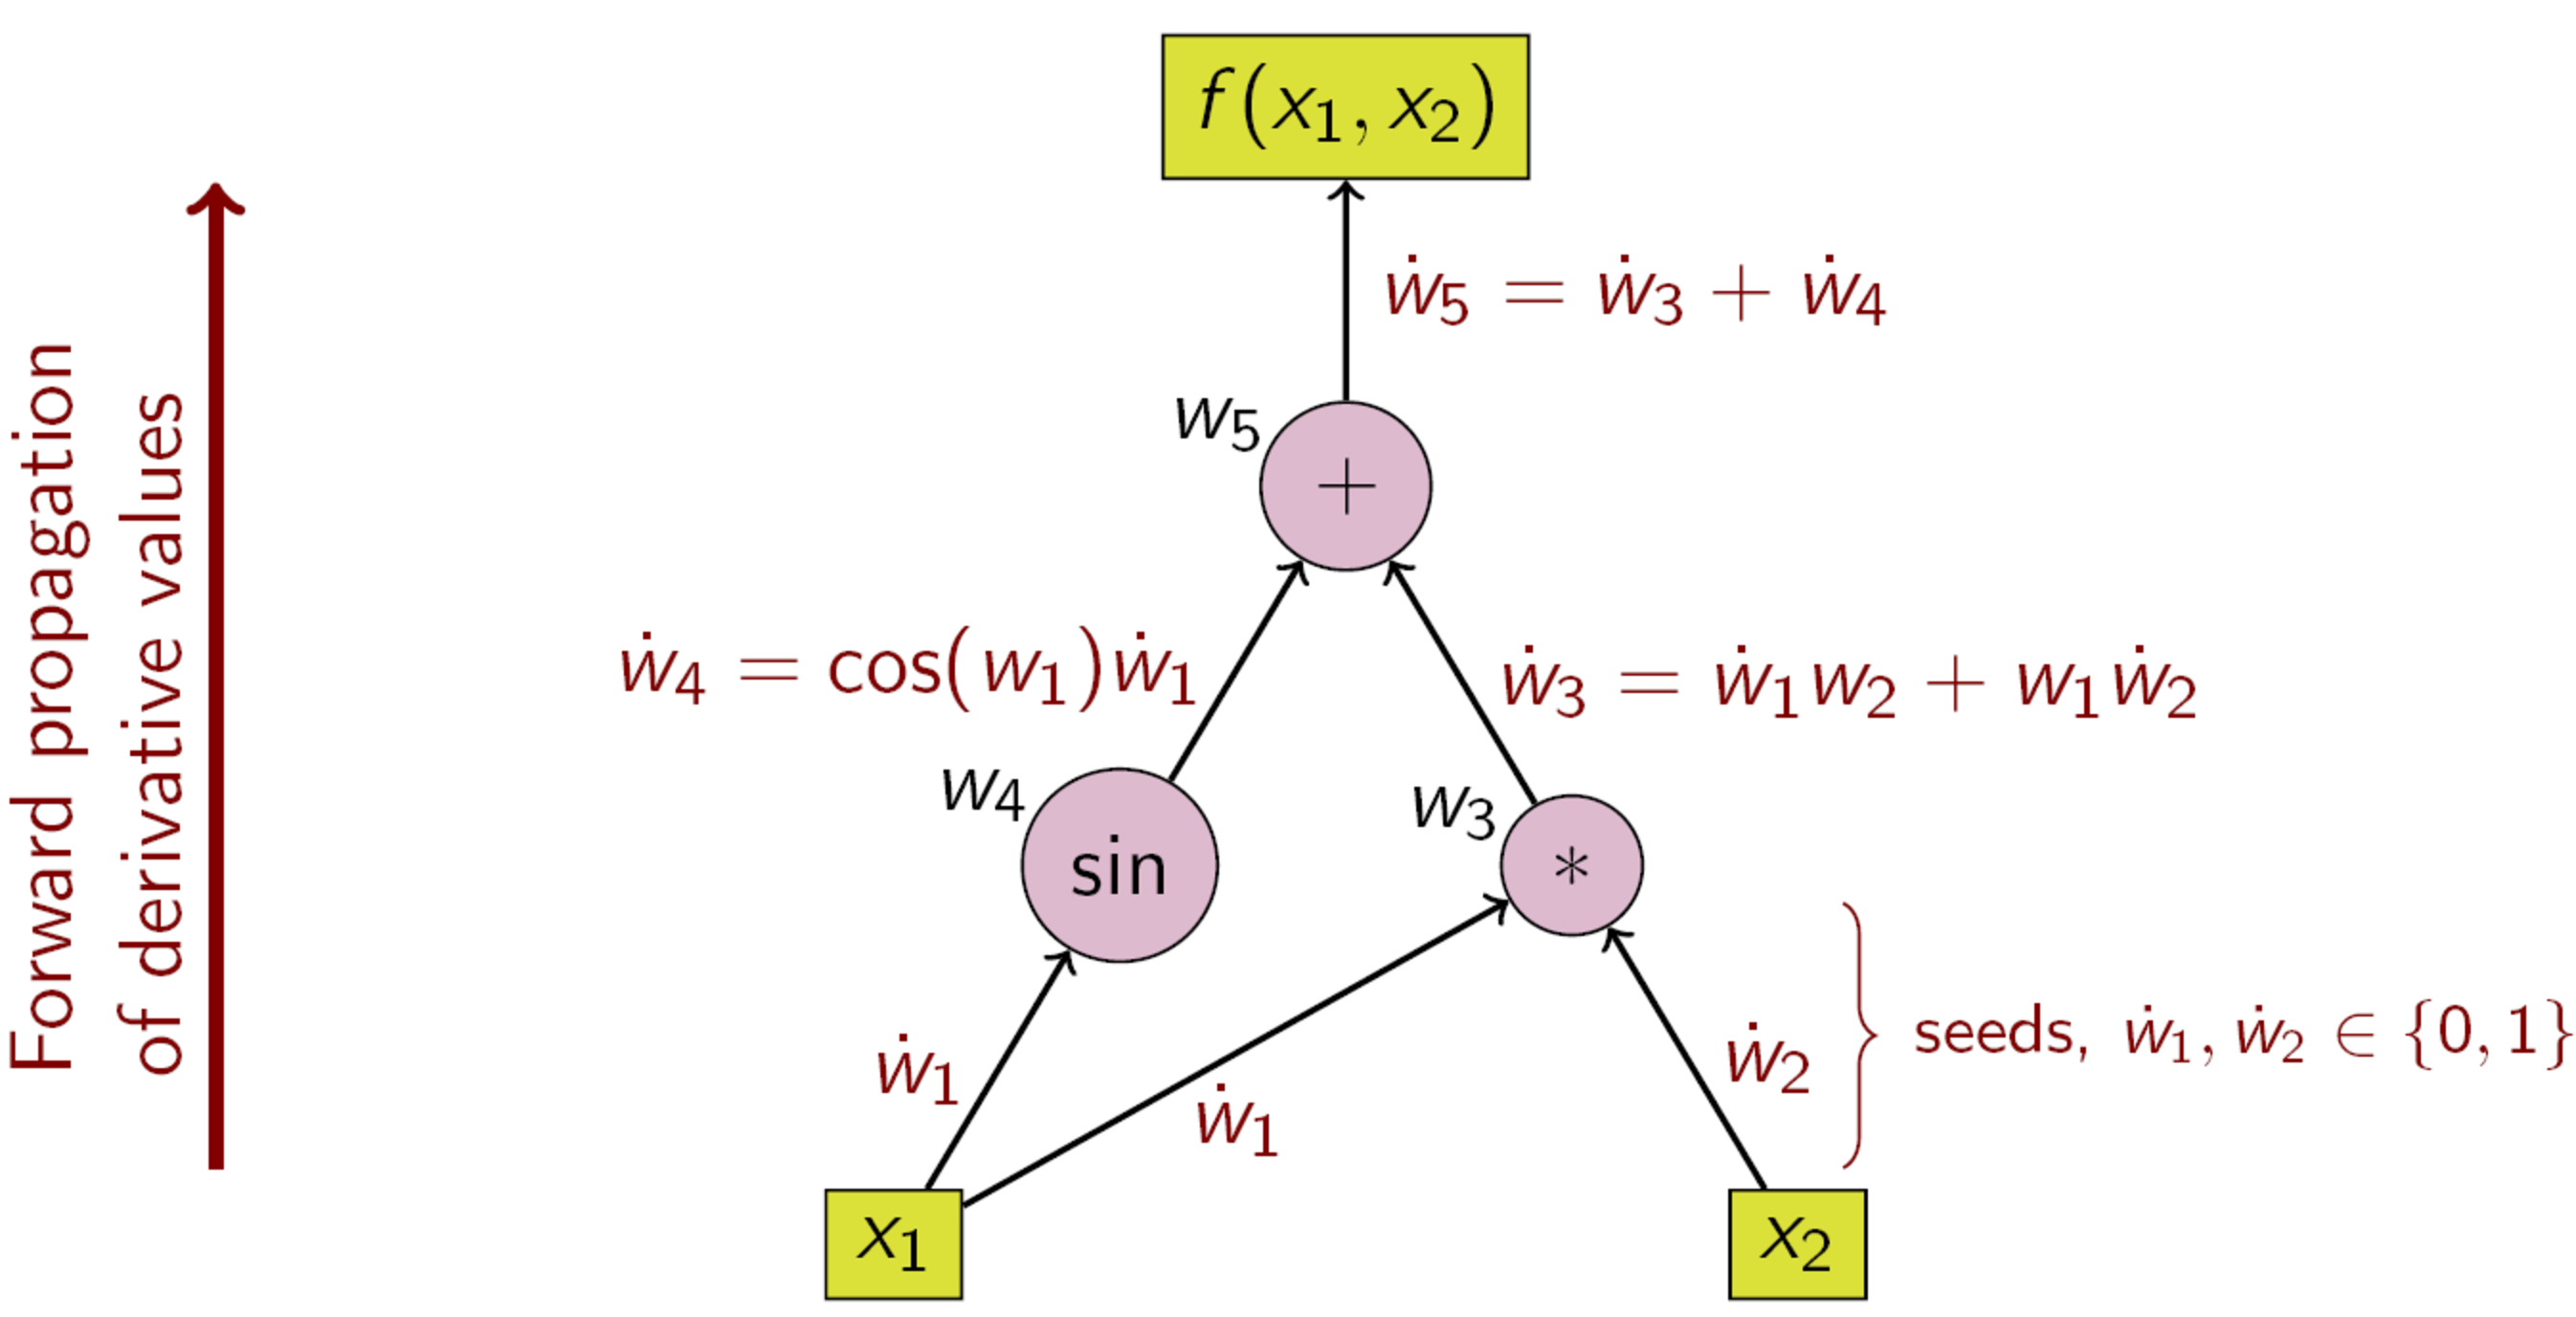
\includegraphics[trim={0cm 0cm 0cm 0cm},clip]{autodiff.pdf}}
       \end{center}
    \end{figure}

\end{frame}


\begin{frame}

    A systematic approach for \brown{computing derivatives of functions
    expressed as computer programs}

        \vspace{0.5em}
    Core idea:

        \vspace{0.5em}
    \begin{enumerate}
        \item Apply the chain rule of calculus to break down complex function evaluations into elementary operations
        \vspace{0.5em}
        \item Compute derivatives by combining the derivatives of these elementary pieces
    \end{enumerate}

        \vspace{0.5em}
        \vspace{0.5em}
        \vspace{0.5em}
        Outcome: \brown{Exact, efficient, automated}

\end{frame}

\begin{frame}[fragile]
    
    
    \begin{minted}{python}
# Set learning rate
λ = 0.01

# Define function to minimize
def f(θ):
  return jnp.sum(θ**2)

# Set up gradient function 
Df = grad(f)

# Update current guess
θ = θ - λ * Df(θ)
    \end{minted}

\end{frame}

\begin{frame}[fragile]
    \frametitle{Just-in-time compilers}

    \vspace{0.5em}
    
    \begin{minted}{python}
@jax.jit
def f(x):
    return jnp.sin(x) - jnp.cos(x**2)
    \end{minted}

    \vspace{0.5em}
    \vspace{0.5em}
    Advantages over traditional (AOT) compilers:

    \begin{itemize}
        \item cleaner code 
    \vspace{0.5em}
        \item more portable
    \vspace{0.5em}
        \item lower compile times -- only compile as required
    \vspace{0.5em}
        \item automatic parallelization (same code for CPUs / GPUs)
    \end{itemize}

\end{frame}



\begin{frame}
    \frametitle{Platforms}
    
    Platforms that support AI / deep learning:

    \vspace{0.5em}
    \begin{itemize}
        \item \brown{Tensorflow}
        \vspace{0.5em}
        \item \brown{PyTorch} (Llama, ChatGPT)
        \vspace{0.5em}
        \item \brown{Google JAX} (Gemini, DeepMind)
        \vspace{0.5em}
        \item \brown{Keras} (backends $=$ JAX, PyTorch, Tensorflow)
    \end{itemize}

\end{frame}


\begin{frame}
    
    Popularity -- DL frameworks
    
    \begin{figure}
       \begin{center}
        \scalebox{0.62}{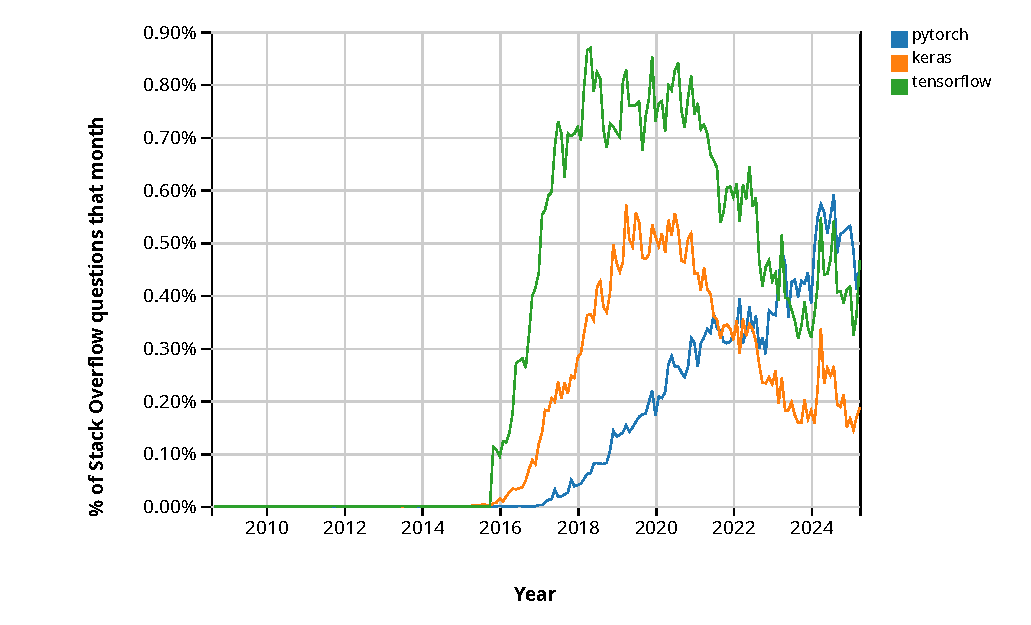
\includegraphics[trim={0cm 0cm 0cm 0cm},clip]{trends_2.pdf}}
       \end{center}
    \end{figure}

\end{frame}

\begin{frame}
    
    Popularity -- languages and libraries
    
    \begin{figure}
       \begin{center}
        \scalebox{0.62}{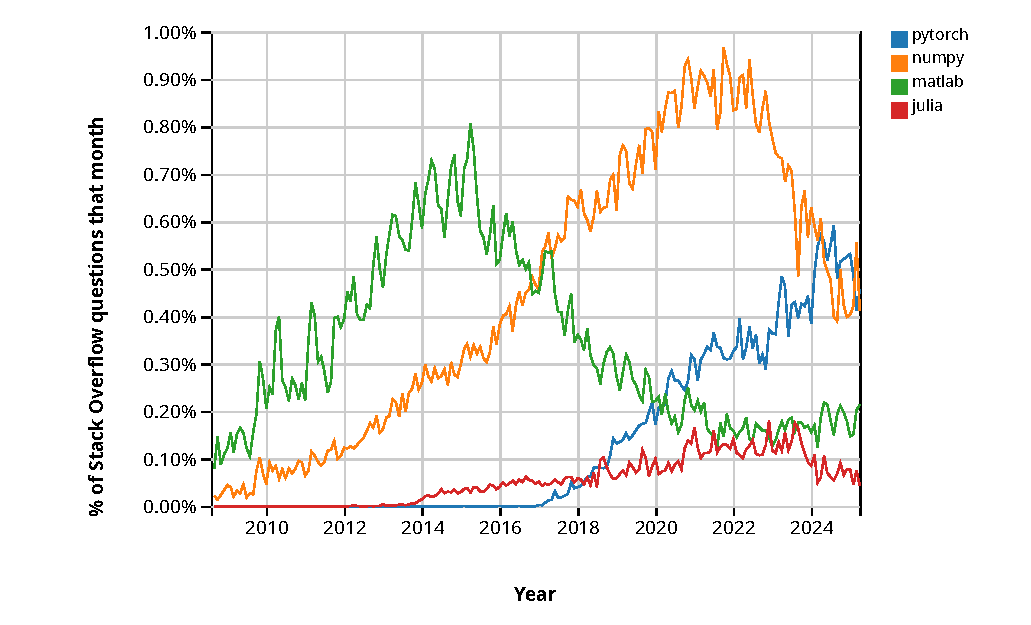
\includegraphics[trim={0cm 0cm 0cm 0cm},clip]{trends.pdf}}
       \end{center}
    \end{figure}

\end{frame}


\begin{frame}

    I mainly use

            \vspace{0.5em}

    \begin{figure}
       \centering
       \scalebox{0.2}{
\includegraphics{logo.pdf}}
    \end{figure}
    
            \vspace{0.5em}

    \begin{itemize}
        \item Developed by Google Research
            \vspace{0.5em}
        \item Rising popularity
            \vspace{0.5em}
        \item Elegant design that exposes low level routines
    \end{itemize}

\end{frame}


\begin{frame}

    ``The acronym JAX stands for \brown{Just After eXecution}''

    \begin{itemize}
        \item monitor function execution once and then compile
    \end{itemize} 

            \vspace{0.5em}
            \vspace{0.5em}
            \vspace{0.5em}

    Another acronym:

    \begin{itemize}
        \item \brown{J}ust-in-time compilation
            \vspace{0.5em}
        \item \brown{A}utomatic differentiation
            \vspace{0.5em}
        \item \brown{X}LA (accelerated linear algebra)
    \end{itemize}



\end{frame}


\begin{frame}[fragile]

    Some typical JAX code
    
    \begin{minted}{python}
def f(θ, x):
  for W, b in θ:
    w = W @ x + b
    x = jnp.tanh(w)  
  return x

def loss(θ, x, y):
  return jnp.sum((y - f(θ, x))**2)

grad_loss = jit(grad(loss))  
    \end{minted}

\end{frame}


\begin{frame}
    \frametitle{AI tools for economic modeling}

    Is DL well-suited to economic modeling?

    \medskip

    \Eg Is macro-forecasting similar to weather forecasting?

    \medskip
    \medskip

    Why or why not?

\end{frame}




\begin{frame}{Repurposing AI tools}
    
    Let's say that you want to do standard macro modeling (not DL)

    \vspace{0.5em}
    Can these new AI tools be applied?

    \pause

    \vspace{0.5em}
    \vspace{0.5em}
    \emp{Yes!}
    \emp{Yes!}
    \emp{Yes!}

    \begin{itemize}
        \item fast matrix algebra
        \vspace{0.5em}
        \item fast solutions to linear systems
        \vspace{0.5em}
        \item fast nonlinear system solvers
        \vspace{0.5em}
        \item fast optimization, etc.
    \end{itemize}

\end{frame}



\begin{frame}
    \frametitle{Case Study}

    The CBC uses the ``overborrowing'' model of Bianchi (2011)

    \begin{itemize}
        \item credit constraint loosens during booms
        \item bad shocks $\to$ sudden stops
    \end{itemize}

    \vspace{0.5em}
    CBC implementation in MATLAB 

    \begin{itemize}
        \item runs on \$10,000 mainframe with 356 CPUs and 1TB RAM
        \item runtime $=$ 12 hours
    \end{itemize}

    \pause
    \vspace{0.5em}
    Rewrite in Python + Google JAX

    \begin{itemize}
        \item runs on \$400 gaming GPU with 10GB RAM
        \item runtime $=$ 7 seconds
    \end{itemize}


\end{frame}


\begin{frame}{Summary}

    \begin{itemize}
        \item We are witnessing an AI revolution
        \medskip
        \item This revolution is changing scientific research
        \medskip
        \item What impact on comp econ?
    \end{itemize}

        \medskip
        \medskip

    At minimum, we can immediately use
    %
    \begin{enumerate}
        \item AI coding agents --- \brown{use Python}
        \medskip
        \item AI software for traditional comp econ --- \brown{use JAX}
        \medskip
        \item AI hardware for traditional comp econ --- \brown{use GPUs}
    \end{enumerate}


\end{frame}


\end{document}


